% !TeX spellcheck = en_GB
\documentclass[
 paper=A4,pagesize=automedia,fontsize=12pt,
 BCOR=15mm,DIV=22,
 twoside,headinclude,footinclude=false,
 fleqn,                     % fleqn = linksbündige Ausrichtung von Formeln
 bibtotocnumbered,          % Literaturverz. im Inhaltsverz. eintragen
 liststotoc,                % Abbildungsverz. im Inhaltsverz. eintragen
 listsleft,                 % Abbildungsverz. an der längsten Nummer ausrichten
 %pointlessnumbers,          % kein Punkt nach Überschriftsnummerierung
 cleardoublepage=empty      % Vakatseiten ohne Paginierung
]{scrbook}
\setlength\parindent{0em}

% Kodierung, Schrift und Sprache auswählen
\usepackage[utf8]{inputenc}
\usepackage[T1]{fontenc}
\usepackage{babel}
% damit man Text aus dem PDF korrekt rauskopieren kann
\usepackage{cmap}
% Layout: Kopf-/Fußzeilen, anderthalbfacher Zeilenabstand
\usepackage{scrpage2} \pagestyle{scrheadings}
                      \clearscrheadfoot
                      \ihead{\headmark}\ohead{\pagemark}
                      \automark[subsection]{section}
                      \setheadsepline{0.5pt}
\usepackage{setspace} \onehalfspacing
\deffootnote{1em}{1em}{\textsuperscript{\thefootnotemark }}
% Grafiken, Tabellen, Mathematikumgebungen
\usepackage{graphicx,xcolor}
\usepackage{tabularx}
\usepackage{amsmath,amsfonts,amssymb}
% Darstellung von Fließumgebungen
\usepackage{flafter,afterpage}
\usepackage[section]{placeins}
\usepackage[margin=8mm,font=small,labelfont=bf,format=plain]{caption}
\usepackage[margin=8mm,font=small,labelfont=bf,format=plain]{subcaption}

\numberwithin{equation}{chapter}
\numberwithin{figure}{chapter}
\numberwithin{table}{chapter}

%%%%%%%%%%%%%%%%%%%%%%%%%%%%%%%%%%%%%%%%%%%%%%%%%%%%%%%%%%%%%%%%%%%%%%%%%%%%%%%%
% Ab hier ist Platz für eigene Ergänzungen (Pakete, Befehle, etc.)

% Dieses Paket liefert den Blindtext, der als Platzhalter in den Beispieldateien steht.
% Das kannst Du also entfernen, wenn Du den Blindtext nicht mehr brauchst.
\usepackage{lipsum}
%\usepackage{ bbold }
\usepackage{physics}
\usepackage{svg}
\usepackage{yfonts}
\usepackage{dsfont}
\begin{document}

\frontmatter


% Titelpageseite
\begin{titlepage}
 \begin{tabularx}{\linewidth}{X}
  
\includegraphics[width=6cm]{TU_Logo_SW} \\\hline\hline

  \vspace{4.5em}

  \begin{singlespace}\begin{center}\bfseries\Huge
  
  Title of Bachelor thesis
  
  \end{center}\end{singlespace}

  \vspace{5.5em}

  \begin{singlespace}\begin{center}\large
   Bachelor-Arbeit \\ zur Erlangung des Hochschulgrades \\ 
   Bachelor of Science \\ 
   im Bachelor-Studiengang Physik
  \end{center}\end{singlespace}\medskip

  \begin{center}vorgelegt von\end{center}
  \begin{center}
   {\large Felix Soest} \\ geboren am 16.09.1998 in Düsseldorf
  \end{center}\medskip

  \begin{singlespace}\begin{center}\large
   Institut für Theoretische Physik \\
   Fakultät Physik \\
   Bereich Mathematik und Naturwissenschaften \\
   Technische Universität Dresden \\ 2021
  \end{center}\end{singlespace}
 \end{tabularx}
\end{titlepage}


% Gutachterseite
\thispagestyle{empty}\vspace*{48em}

Eingereicht am xx.~Monat~20xx\vspace{1.5em}
\par{\large\begin{tabular}{ll}
 1. Gutachter: & Prof.~Dr.~Walter~Strunz \\
 2. Gutachter: & Prof.~Dr.~Oscar~Dahlsten \\
\end{tabular}}


% Abstractseite
\newpage
\begin{center}\large\bfseries Summary\end{center}


Abstract \\ 
English: \\
Aufmerksamkeit
große Fragen?
unsere Frage
unsere Antwort

\vspace{20em}
Abstract \\ 
Deutsch \\
 
 
% Inhaltsverzeichnis
%\cleardoublepage
\tableofcontents



% Hauptteil
\mainmatter

\chapter{Introduction}

\section{Intro}
% !TeX root = ../BA_main_englisch.tex
% !TeX spellcheck = en_GB
Thermodynamics has been a central field of interest in physics ever since its inception in the 19th century \cite{thomson_2011}.

Due to the increasing availability of data and computing power, machine learning methods have become a standard approach in many fields such as natural language processing \cite{DBLP:journals/corr/VaswaniSPUJGKP17}.
Additionally, these methods are being applied to a broad range of problems in the physical sciences, from statistical physics to quantum computing \cite{Carleo_2019, wise2021using}.

Machine learning has also found use in the field of energy harvesting, concerned with extracting energy from external excitations, e.g. vibrations in human motion \cite{Liu2019}.
In this work we extend this concept to the quantum case.
Work extraction is often modelled as a system coupled to a heat bath, and bounds for the extractable work exist \cite{Egloff_2015}.
We take a different approach, following the framework given in \cite{beyer2020}.
We examine a system that can be driven by an arbitrary excitation, modelled as a time-dependent system Hamiltonian.
The transducer is modelled in a similar fashion and can extract work from the system.
By following a policy of local optimisation of the work output, we show that a lower bound of the extractable work exists for specific initial conditions.
We train neural networks to predict transducer protocols given a drive sequence, considering both the case where the sequence is known beforehand and the one where it is not.

The remainder of this work is structured as follows.
In Chapter \ref{background} we review the collision model framework used in our approach and introduce two machine learning architectures.
In Chapter \ref{lower_bound} we show that for a given drive sequence a lower bound on the expectation value of the extractable work exists.
We investigate the system under consideration in Section \ref{dep_dt} and apply the aforementioned architectures in Sections \ref{n_2_ml} to \ref{work_cost}.
We summarise our findings and provide an outlook in Chapter \ref{outlook}.

We use units where $\hbar = 1$.

\chapter{Background}
\section{Supervised Machine Learning} \label{sml}
Machine learning is a subfield of artificial intelligence, `concerned with the question of how to construct computer programs that automatically improve with experience.' \cite{Mitchell97}
Supervised machine learning is one of the three machine learning disciplines, besides unsupervised and reinforcement learning.
The goal is to find a mapping between an input and an output, in our case an excitation and its respective optimal harvesting policy.
Multiple algorithms to find such a mapping exist, however for high dimensional problems artificial neural networks (ANNs) are usually used.
In the following sections we review two ANN architectures, the fully-connected feedforward ANN and the Long Short-Term Memory (LSTM) network.

\subsection{Fully-connected feedforward ANNs}
In this section we review ANNs, following the exposition given in \cite{lu2020dying}.
Let $\textfrak{N}$ be a fully-connected feedforward ANN, meaning there are no loops in the neuron connections and all neurons in a layer are connected to every neuron of the next layer, $\textfrak{N}: \mathbb{R}^{n_1} \to \mathbb{R}^{n_L}$. $n_1$ and $n_L$ denote the dimensionality of the input and output respectively. 
$\textfrak{N}$ has $L$ layers, or columns of neurons.
The network architecture is given by the amount of neurons $n_l$ in each hidden layer $l \in [2, L - 1]$ (see figure \ref{nn}).
The neurons in layer $l$ are represented by their activations $\vec{a}_l \in \mathbb{R}^{n_l}$, which represent the matrix multiplication output. Additionally each layer includes trainable parameters $W_l \in \mathbb{R}^{n_{l+1} \times n_{l}}$ and $\vec{b}_l \in \mathbb{R}^{n_l}$ called weights and biases.
The activations can then be calculated using the following formulae \cite{TN_libero_mab2)53517}:
\begin{align*}
	\vec{a}_2 & = W_1 \vec{a}_1 + \vec{b}_1, \\
	\vec{a}_l & = W_{l-1} \xi(\vec{a}_{l-1}) + \vec{b}_{l-1}, \ l \in [3, L],
\end{align*}
where $\xi(x)$ is a function called the activation function applied elementwise. Historically, functions such as $\tanh$ and sigmoid have been used. However, it has been shown \cite{Maas2013RectifierNI, krizhevsky} that the rectified linear unit $\mathrm{ReLU}(x) = \mathrm{max}(0, x)$ often provides better results and is used here.


\subsection{Long Short-Term Memory}
While the network architecture introduced in the previous section performs reasonably well on many problems, it destroys spatial and temporal correlations present in the data. 
Instead convolutional and recurrent networks are often used for these purposes, e.g. in image recognition and time series forecasting \cite{rumelhart1986learning, 10.1007/978-3-642-46466-9_18}.

Here we use the LSTM architecture, a type of recurrent neural network (RNN) introduced in \cite{doi:10.1162/neco.1997.9.8.1735}. 
The core idea of RNNs is the usage of loops to store and propagate information through time.

The network is made up of a row of LSTM cells which share parameters.
The cell uses the current input $x_t$ as well as the previous cell state $c_{t-1}$ and output $h_{t-1}$ to compute the output $h_t$.
Internally, the cell is comprised of multiple gates which control the storage of information, $i_t, f_t, g_t, o_t$, which are the input, forget, cell and output gates respectively.
The output and gates of each cell are computed using the following equations:
\begin{align*}
i_t & = \sigma (W_{ii} x_t + b_{ii} + W_{hi} h_{t-1} + b_{hi}), \\
f_t & = \sigma (W_{if} x_t + b_{if} + W_{hf} h_{t-1} + b_{hf}), \\
g_t & = \tanh (W_{ig} x_t + b_{ig} + W_{hg} h_{t-1} + b_{hg}), \\ 
o_t & = \sigma (W_{if} x_t + b_{if} + W_{hf} h_{t-1} + b_{hf}), \\
c_t & = f_t \odot c_{t-1} + i_t \odot g_t, \\
h_t & = o_t \odot \tanh (c_t).
\end{align*}

\subsection{Training \& Backpropagation}
To train an ANN a cost function is defined, often the mean squared error 
\begin{align*}
	\mathrm{MSE} = \frac{1}{N} \sum_{i=1}^N (\vec{a}_{L, i} - \vec{y}_i)^2,
\end{align*}
where the summation is performed over the training data $\{(\vec{x}_i, \vec{y}_i)\}$ with $N$ samples, where $\{\vec{x_i}\}$ is the input and $\{\vec{y_i}\}$ the output data, and $\vec{a}_{L, i} = \textfrak{N}(\vec{x}_i)$ is the output of the neural network.
The so-called backpropagation algorithm is used to calculate the gradient of the cost function with respect to the trainable parameters and improve the performance of the ANN \cite{rumelhart1986learning, nielsenneural}.

\begin{figure}
	\centering
	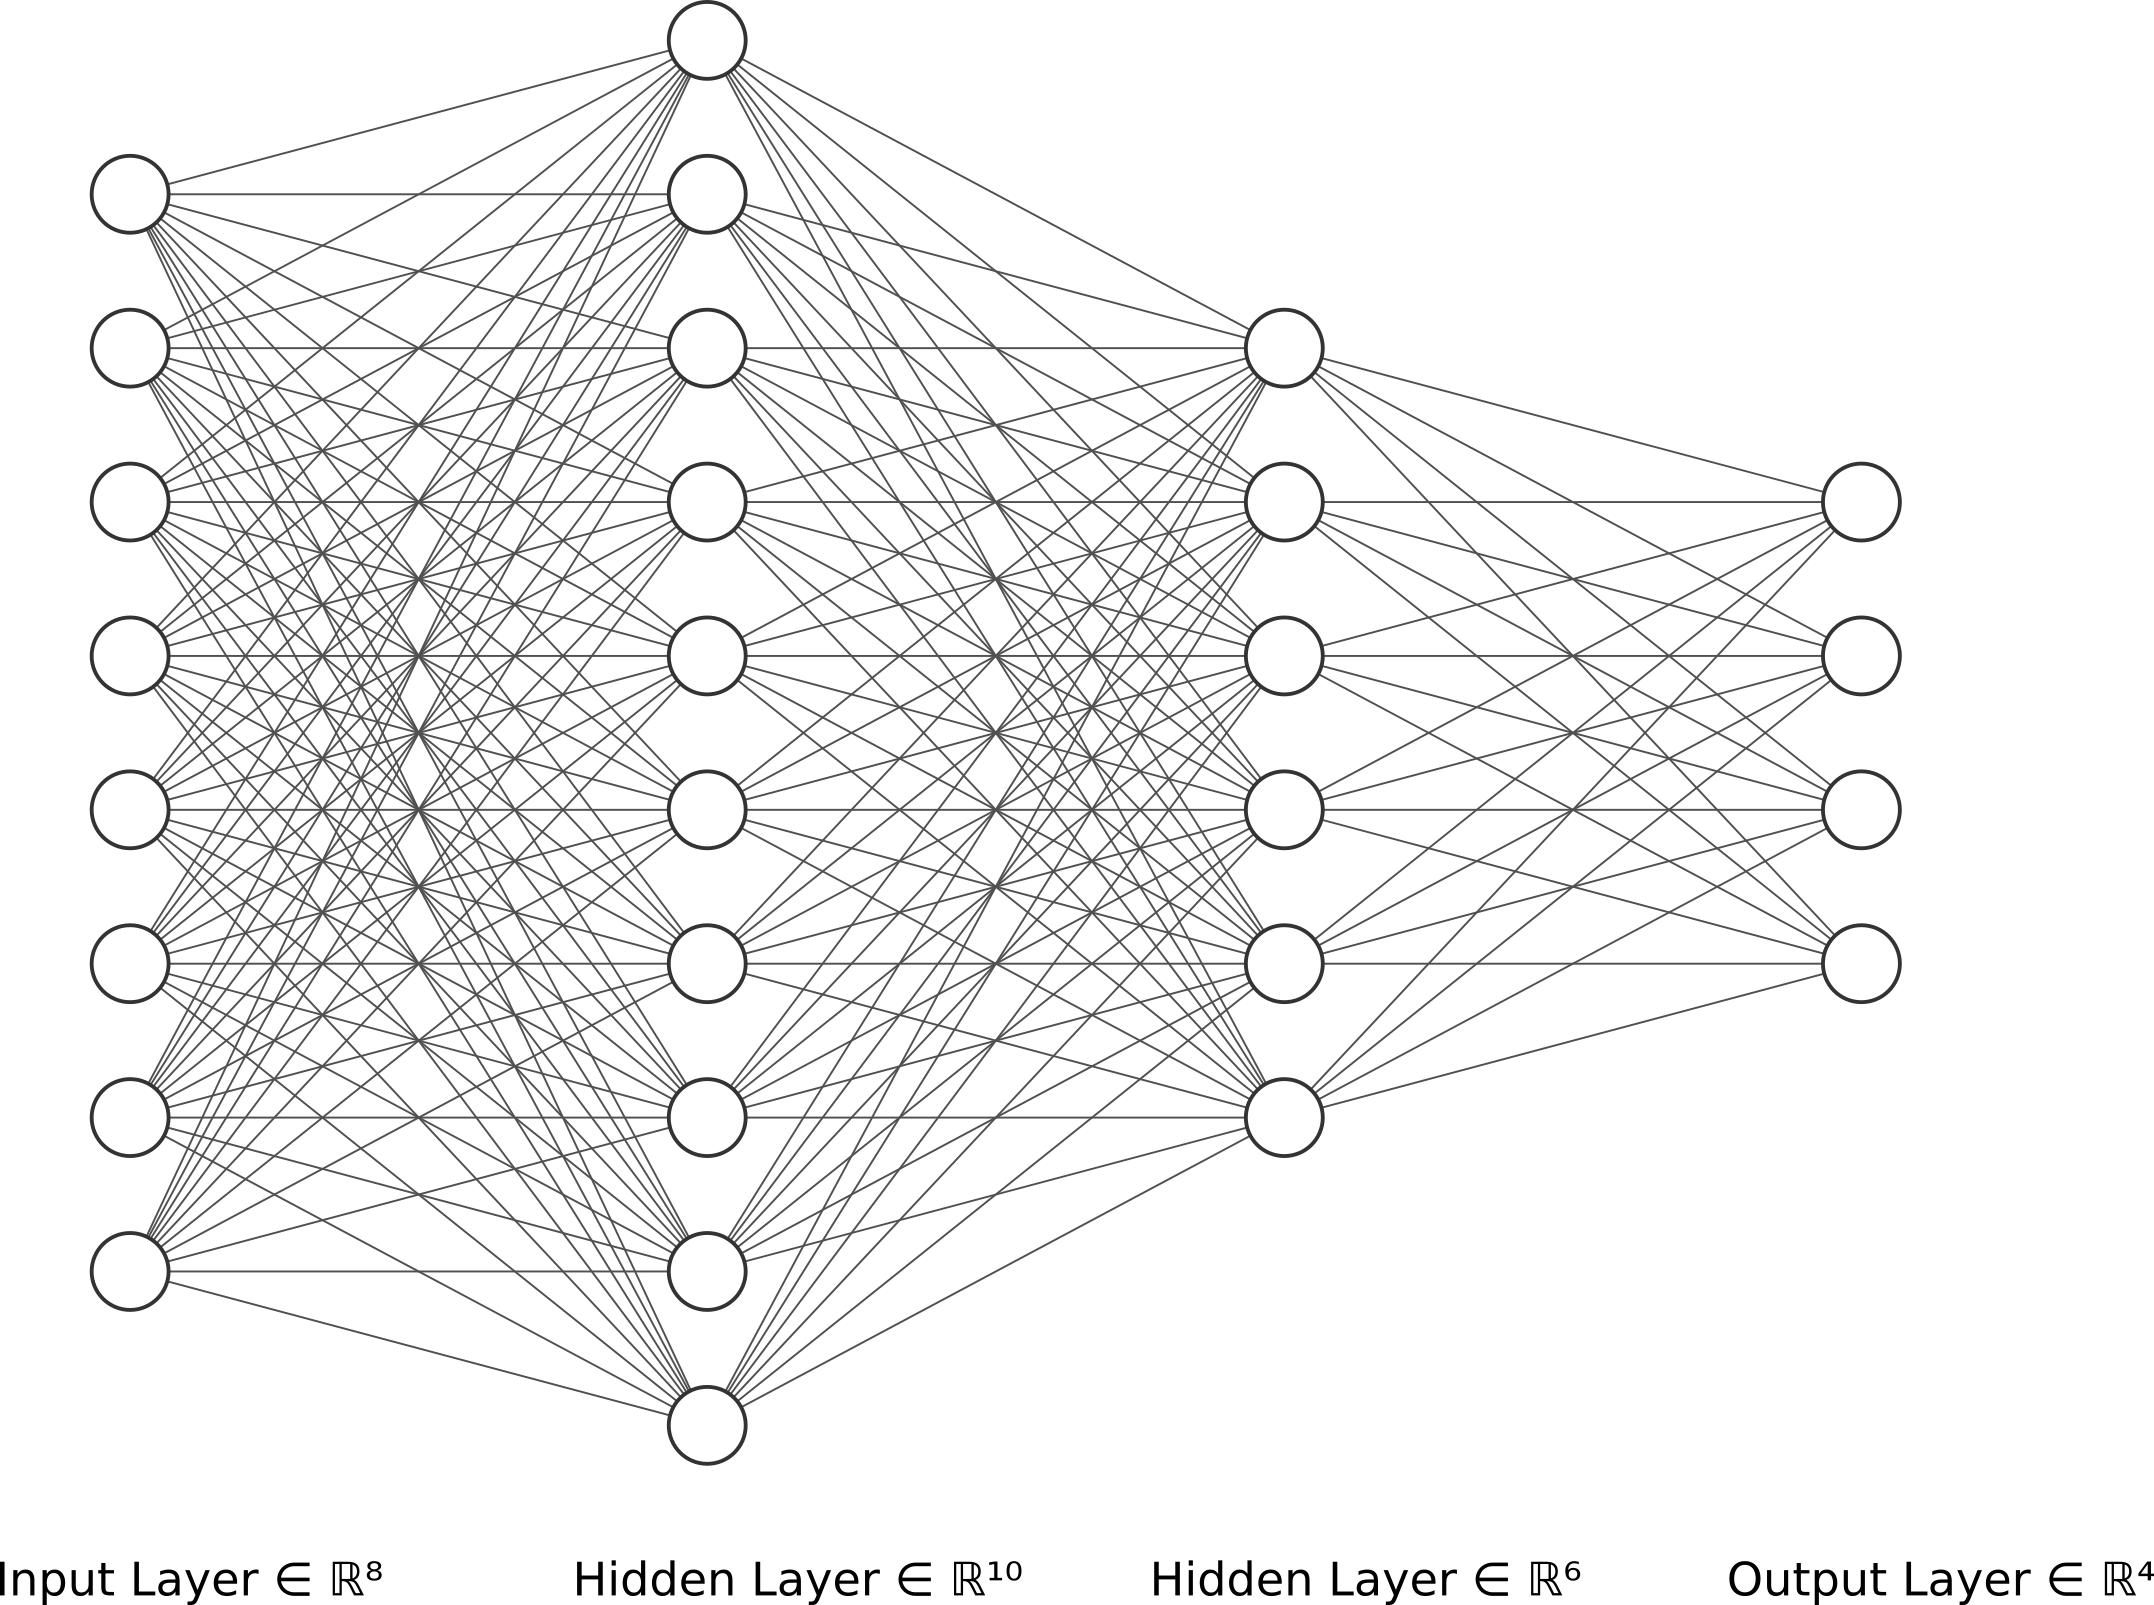
\includegraphics[width=0.6\textwidth]{img/nn}
	\caption{Example fully-connected feedforward ANN with four layers, including input, output and two hidden layers \cite{LeNail2019}}.
	\label{nn}
\end{figure}



\section{Collision model dynamics} \label{col_model}
% !TeX spellcheck = en_GB
A standard approach to modelling open quantum systems is the collision model.
The system under consideration interacts with a series of ancilla systems through a unitary transformation on the combined system-ancilla state \cite{Lorenzo_2017}. After a short interaction time $\Delta t$, the ancilla systems are traced out to receive the system state.
This type of interaction will in general lead to entanglement between system and ancilla.
This is undesirable in our setting, the reason for which will become apparent in the next paragraph.
To ensure the ancilla and system states remain pure, we follow the approach used in \cite{beyer2020}:
let $\rho_S$ be the density operator of the system under consideration and $\ket{\psi_A}$ the state of the ancilla system.
Given $\Delta t \ll 1$ the time evolution of $\rho_S$ under $H_{AS}$ acting on the combined system is
\begin{align}\label{coll_eq}
\rho'_S & = \mathrm{Tr}_A \{ e^{-i H_{AS} \Delta t} (\ket{\psi_A} \bra{\psi_A} \otimes \rho_S) e^{i H_{AS} \Delta t} \} & = \rho_S - i \Delta t [\expval{H_{AS}}{\psi_A}, \rho_S] + O(\Delta t^2).
\end{align}

In the continuous limit Eq. (\ref{coll_eq}) leads to von-Neumann dynamics on the system for an infinite stream of qubits initialised in the same state $\ket{\psi_A}$:
\begin{align*}
	\dot{\rho}_S = - i [\expval{H_{AS}}{\psi_A}, \rho_S].
\end{align*}

As each ancilla only interacts once with the system and is traced out afterwards, $\rho_S$ remains pure in the limit of $\Delta t \to 0$.


We use this approach as the implementation for our setting, which consists of three qubits: the drive, system and transducer qubits.
We focus on piece-wise constant (PWC) functions of the drive ($\ket{\psi_D}$) and transducer ($\ket{\psi_T}$) qubits, as it greatly reduces computational complexity.
These are implemented by keeping the stream of ancillas $\ket{\psi_A} = \ket{\psi_D} \otimes \ket{\psi_T}$ constant for time $\Delta \mathrm{T}$ (Figure \ref{collmodel}).
The drive and transducer qubits can be set in N discrete intervals represented by ($\theta_D^n, \phi_D^n$) and ($\theta_T^n, \phi_T^n$) respectively (see Figure \ref{pwc}), the system qubit is initialised in a pure state $\rho_S$.
Here, the necessity for pure ancillas, in this case both drive and transducer qubit, becomes clear, as a mixed drive or transducer state would not be compatible with the PWC approach where we assume the experimenter to be in control of drive and transducer at all times.

In the remainder of this work we use the interaction Hamiltonian on the three qubit Hilbert space
\begin{equation*}
H_{DST} = H_{I} \otimes \mathds{1}_T + \mathds{1}_D \otimes H_{I}, \\
H_{I} = \sigma_{+} \otimes \sigma_{-} + \sigma_{-} \otimes \sigma_{+}.
\end{equation*}
Note that the interaction Hamiltonian itself is constant and the time dependence comes from the change in the stream of ancillas only.
The energy scale of the Hamiltonian is therefore limited and so are the dynamics of the system state $\rho_S$.
The time evolution and work extraction is then calculated as follows, where $\Delta \mathrm{T}$ is time span between qubit switching:
\begin{align}
H_S^n &= \bra{\psi_D^n}\bra{\psi_T^n} H_{DST} \ket{\psi_D^n} \ket{\psi_T^n}, \label{relham}\\
\rho_S &((n+1) \Delta \mathrm{T}) = U_n \ \rho_S(n \Delta \mathrm{T}) \ U^{\dagger}_n, \\
U_n &= e^{-iH_S^n \Delta \mathrm{T}}, \\
W &= - \Sigma_n \Tr{\rho_S(n \Delta \mathrm{T}) \ dH_S^n}, \\
dH_S^n &= \bra{\psi_D^n}\bra{\psi_T^{n+1}} H_{DST} \ket{\psi_D^n} \ket{\psi_T^{n+1}} - \bra{\psi_D^n}\bra{\psi_T^n} H_{DST} \ket{\psi_D^n} \ket{\psi_T^n}.	
\end{align}
Here we use the partial Hamiltonian $H_S^n$ on the system at time step $n \in [1, N - 1]$, as well as corresponding system density matrix $\rho_S(n \Delta \mathrm{T})$.
An advantage of this framework is that the extracted work is available to the experimenter as a quantum observable \cite{beyer2020}.

Using the Bloch sphere representation $\ket{\psi} = \cos(\frac{\theta}{2}) \ket{0} + e^{i \phi} \sin(\frac{\theta}{2})\ket{1}$ to represent drive and transducer qubits reduces Eq. (\ref{relham}) to
\begin{align}
	H_S^n &= \frac{1}{2} \left[\sin(\theta_D^n) e^{i\phi_D^n} + \sin(\theta_T^n) e^{i\phi_T^n}\right] \sigma_{+} + h.c. =  H_{DS} + H_{ST}.
\end{align}

\begin{figure}
	\centering
	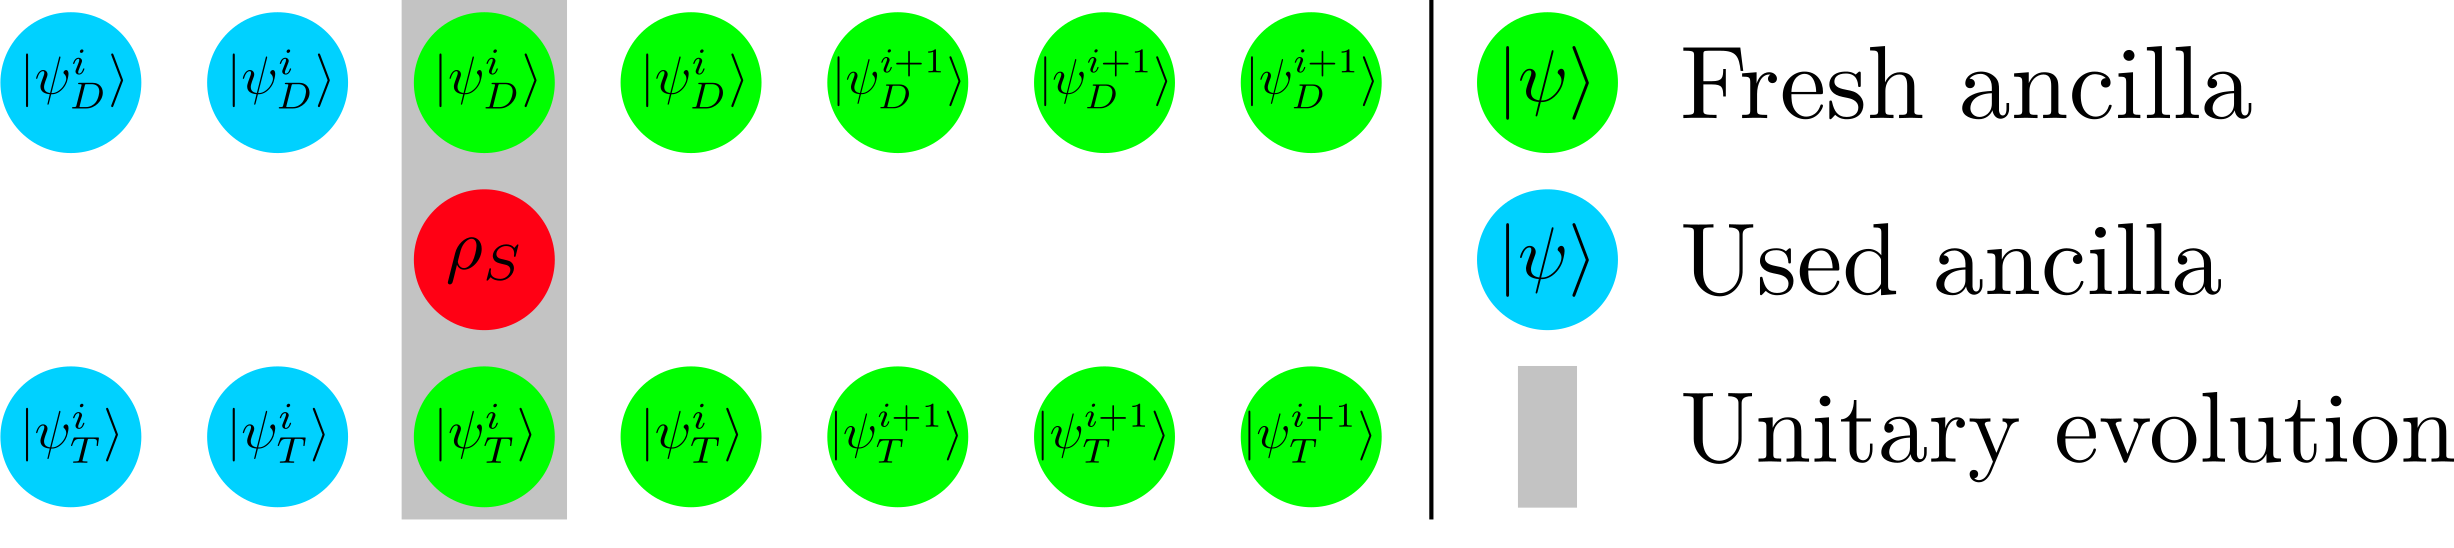
\includegraphics[width=0.85\textwidth]{img/coll2}
	\caption{Collision model used in this work: drive and transducer are series of qubits that interact once with the system and evolve the reduced density operator $\rho_S$. The qubit configuration can be changed in intervals of $\Delta \mathrm{T}$.}
	\label{collmodel}
\end{figure}

\begin{figure}
	\centering
	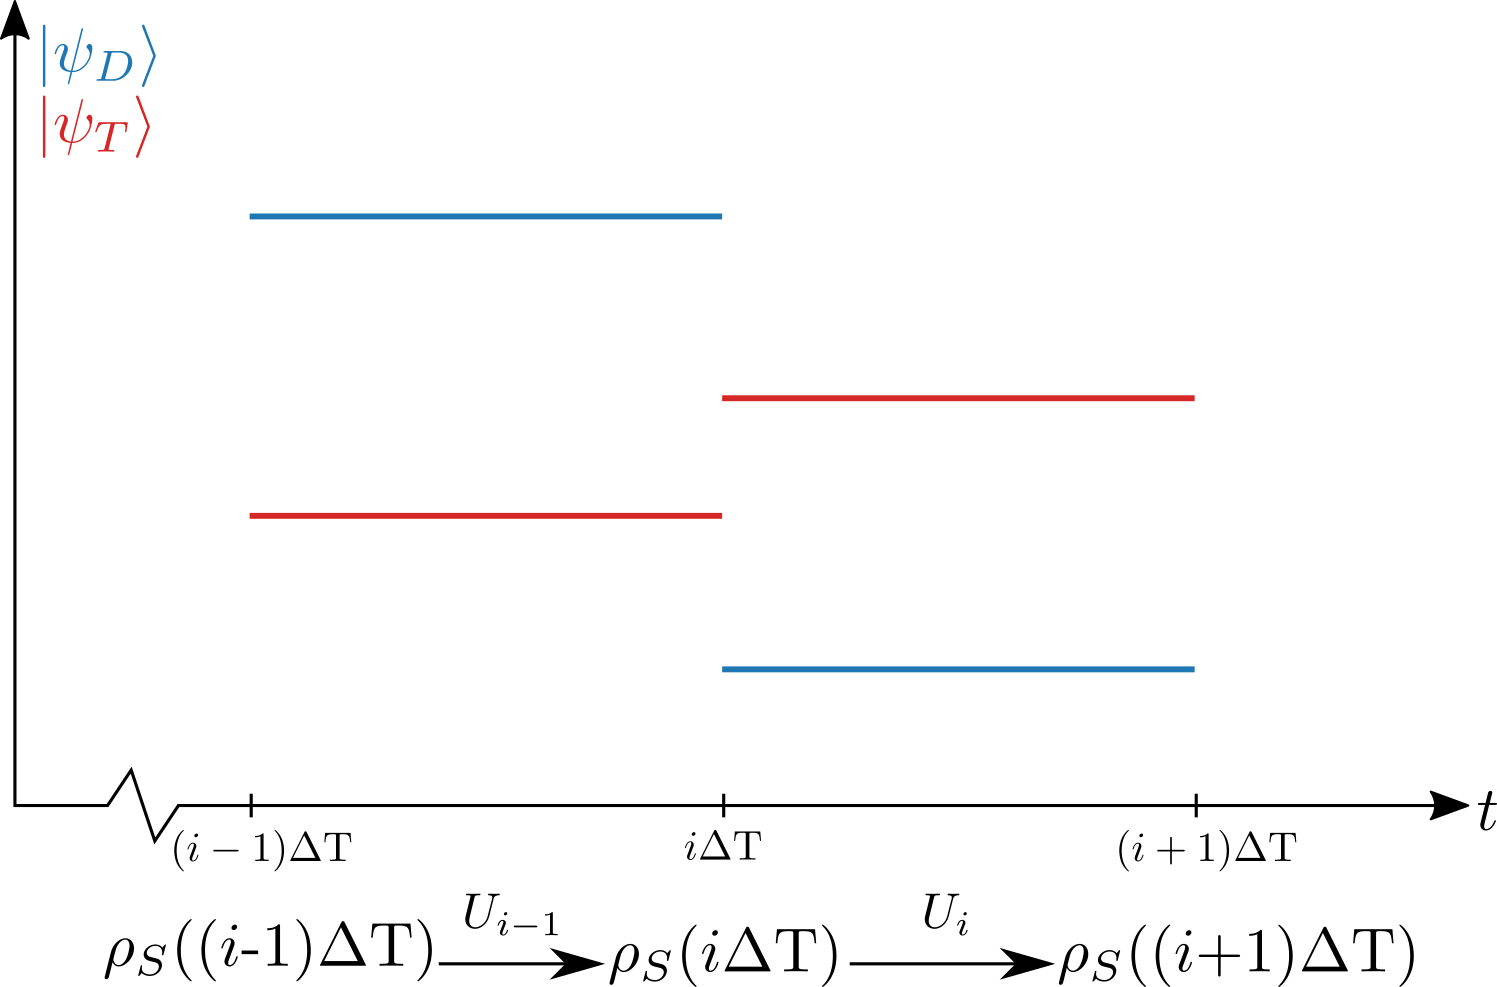
\includegraphics[width=0.6\textwidth]{img/pwc2}
	\caption{Piecewise constant implementation of drive and transducer qubits: the vertical axis represents an arbitrary parameter of the ancilla states. The qubit states are switched instantaneously and then kept constant for $\Delta \mathrm{T}$ while $\rho_S$ evolves unitarily. The piece-wise constant drive and transducer settings lead to a piece-wise constant system Hamiltonian.}
	\label{pwc}
\end{figure}

\section{Setting}
Our setting consists of three qubits: the Drive, System and Transducer qubits. The Drive and Transducer qubits can be set by the experimenter in N discrete steps modelled as piecewise constant functions (PWC) of ($\theta_D, \phi_D$) and ($\theta_T, \phi_T$) respectively (see figure \ref{pwc}), the system qubit is initialised in a pure state.
As Drive and Transducer are assumed to be piecewise constant and therefore pure, we model both qubits as ancillary systems introduced in section \ref{col_model} (see figure \ref{collmodel}).

In the remainder of this work we use the interaction Hamiltonian on the three qubit Hilbert space
\begin{equation*}
	H_{DST} = H_{I} \otimes \mathds{1}_T + \mathds{1}_D \otimes H_{I}, \\
	H_{I} = \sigma_{+} \otimes \sigma_{-} + \sigma_{-} \otimes \sigma_{+}
\end{equation*}
unless otherwise noted.
The time evolution and work extraction is then calculated as follows, where $\Delta \mathrm{T}$ is time span between qubit switching\footnote{It is important to make the distinction between $\Delta \mathrm{T}$ and $\Delta t$ introduced in section \ref{col_model}. $\Delta t$ is the collision time of a single qubit while $\Delta \mathrm{T}$ is the time for which the qubits have the same initial state. For each time step $i$ we therefore have $n = \Delta \mathrm{T} / \Delta t$ qubits initialised in the same state.}:
\begin{align}
	H_S^i = \bra{\psi_D^i}\bra{\psi_T^i} H_{DST} \ket{\psi_D^i} \ket{\psi_T^i} \\
	\rho_S^{i+1} = U^i \rho_S^i U^{i\dagger}, \ U^i = e^{-iH_S^i \Delta \mathrm{T}} \\
	W = - \Sigma_i \mathrm{Tr} \ \rho_S^i \ dH_S^i \\
	dH_S^i = \bra{\psi_D^i}\bra{\psi_T^{i+1}} H_{DST} \ket{\psi_D^i} \ket{\psi_T^{i+1}} - \bra{\psi_D^i}\bra{\psi_T^i} H_{DST} \ket{\psi_D^i} \ket{\psi_T^i}.	
\end{align}
Here we use the partial Hamiltonian $H_S^i$ on S at time step $i \in [1, N - 1]$, as well as corresponding system density matrix $\rho_S^i$.


\begin{figure}
	\centering
	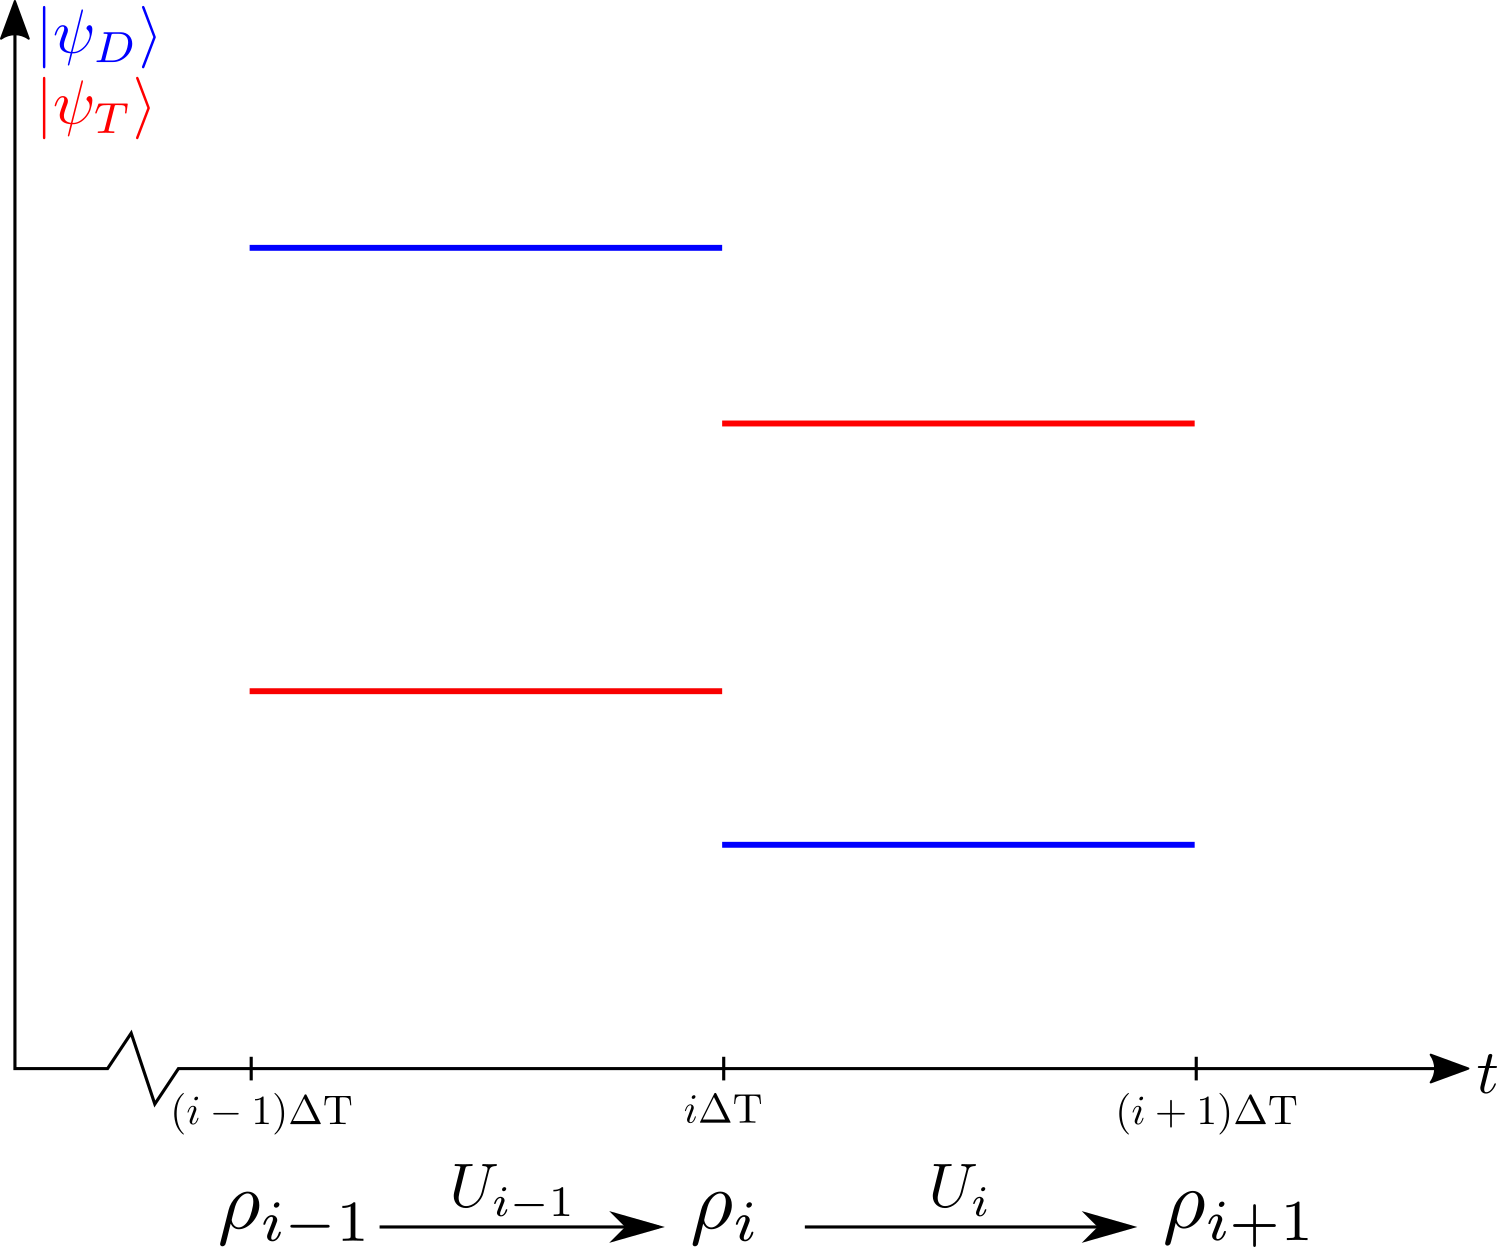
\includegraphics[width=0.6\textwidth]{img/pwc}
	\caption{Piecewise constant implementation of Drive and Transducer qubits: the vertical axis shows qubit state in arbitrary units. The qubit states are switched instantaneously and then kept constant for $\Delta \mathrm{T}$ while $\rho_S$ evolves unitarily.}
	\label{pwc}
\end{figure}

\begin{figure}
	\centering
	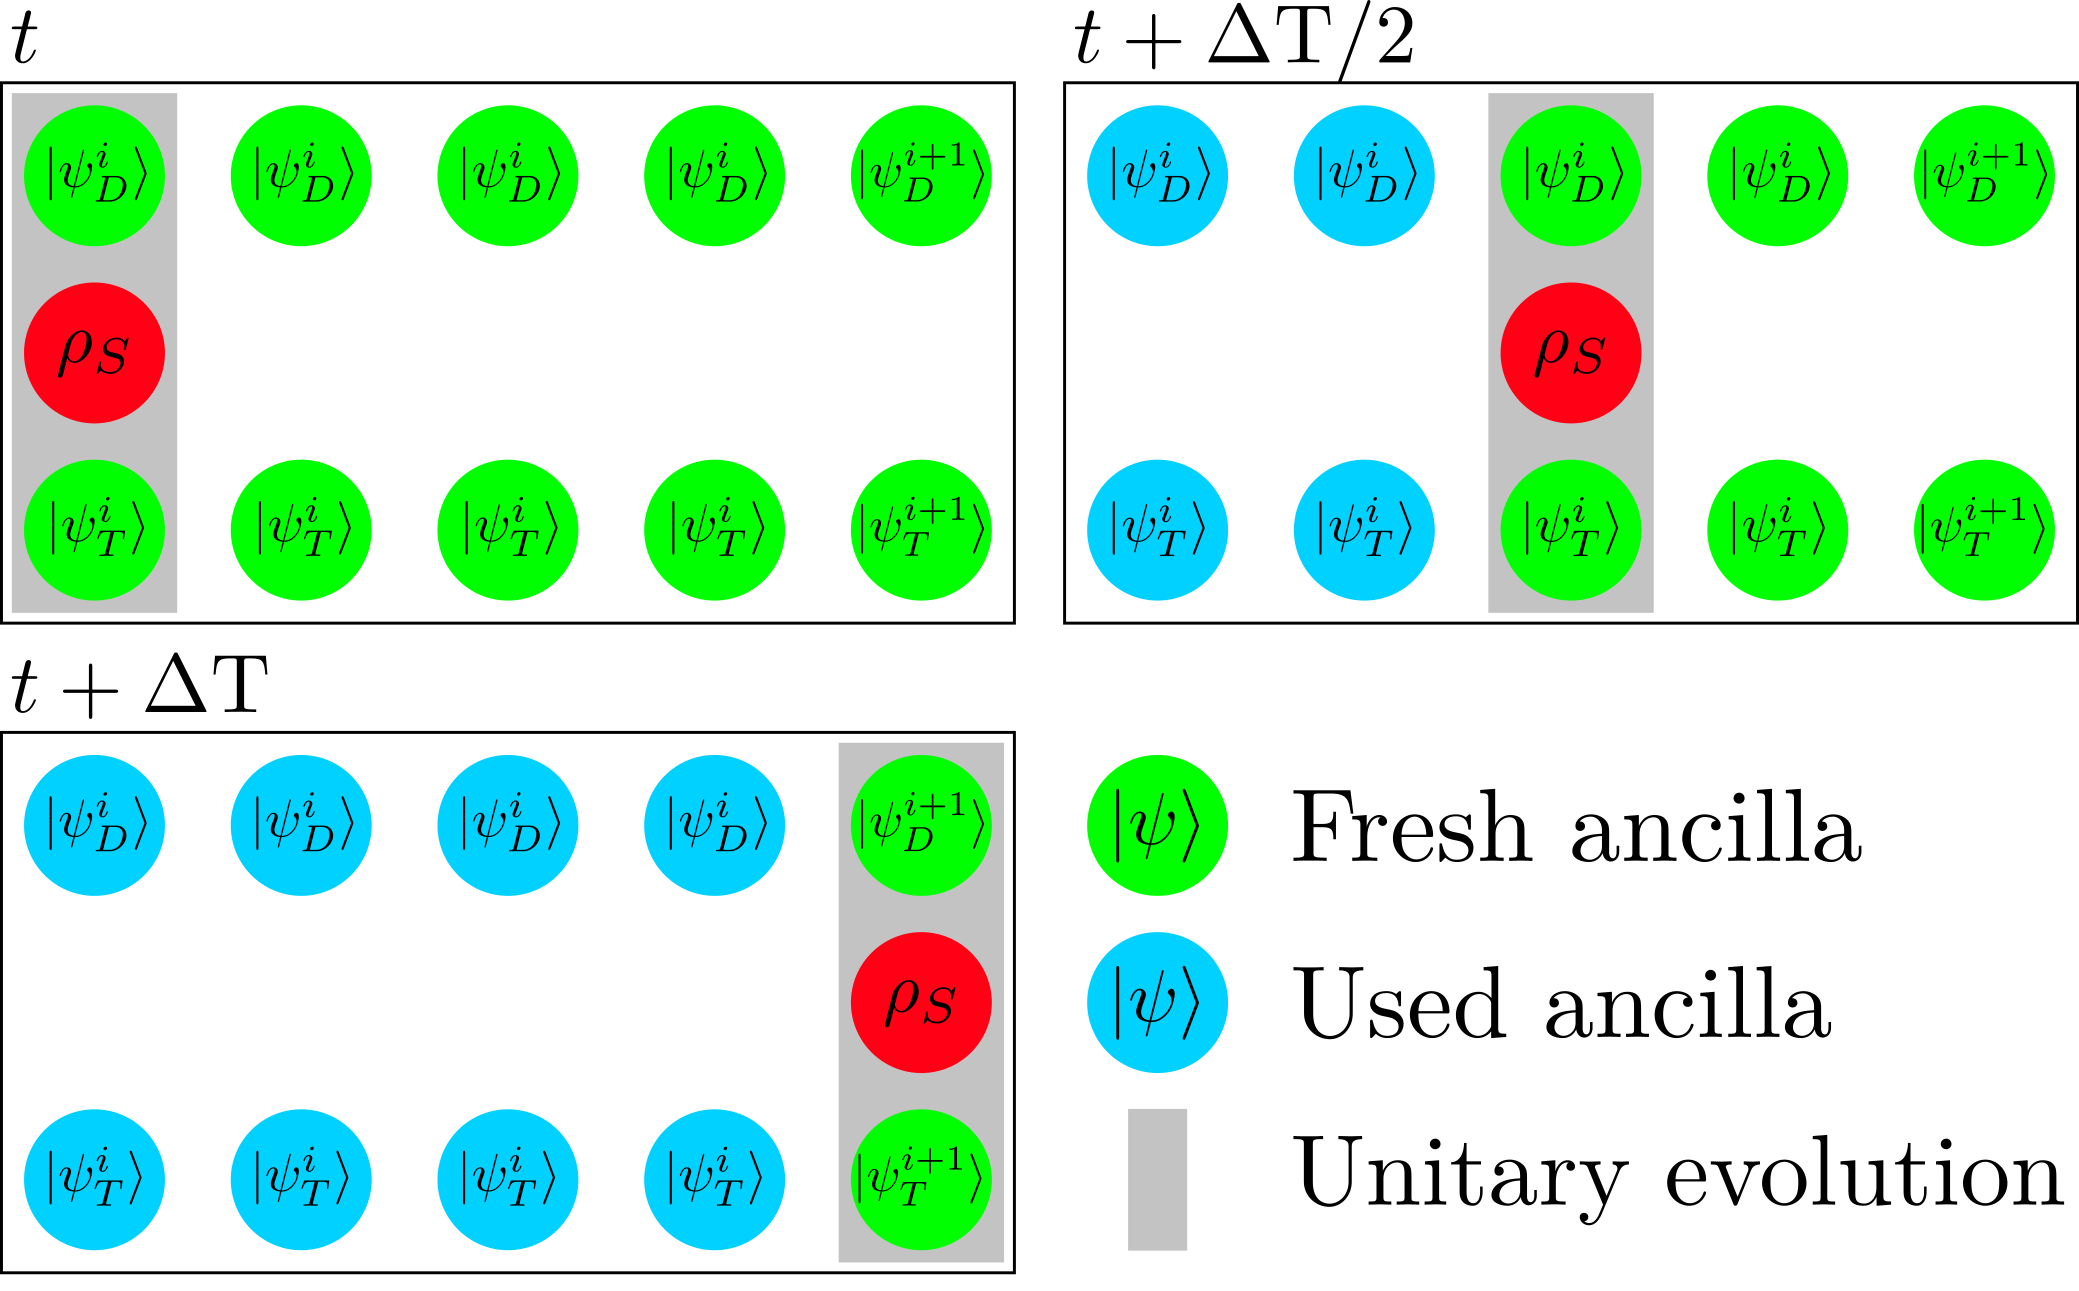
\includegraphics[width=0.7\textwidth]{img/collision_model}
	\caption{Collision model used in this work: Drive and Transducer are series of qubits interact once with the system and evolve the reduced density operator $\rho_S$. The qubit configuration can be changed in intervals of $\Delta \mathrm{T}$.}
	\label{collmodel}
\end{figure}


\chapter{Experimental Results}
The training data is created using a minimisation algorithm \cite{2020SciPy-NMeth}, which finds the optimal transducer protocol $\{|\psi_T^i \rangle\}$ given a drive sequence $\{|\psi_D^i \rangle\}$.
The networks are trained to learn the mapping $\{|\psi_D^i \rangle\} \to \{|\psi_T^i \rangle\}$.
Both the input (drive) and output (transducer) are transformed by the embedding
\begin{align*}
	\left\{
	\begin{pmatrix}
	\theta^n & \phi^n \\
	\end{pmatrix}
	\right\}
	\to
	\left\{
	\begin{pmatrix}
	\sin(\theta^n) & \sin(\phi^n) & \cos(\theta^n)  & \cos(\phi^n) \\
	\end{pmatrix}
	\right\}.
\end{align*}
The reasons for this operation are twofold: it normalises the data to the interval $[-1, 1]$, which is beneficial to learning \cite{LeCun2012}. Additionally it encodes information regarding the periodicity of the qubit angle representation.
We add either a zero or a one as an extra input parameter for LSTM training depending on whether or not the input is the last in a sequence.

To compare the accuracy of different models a performance indicator is required. 
Naturally one might use the MSE as introduced in section \ref{sml}.
Instead we define the \textit{efficiency} of a model $\textfrak{N}$ on a dataset $\{(\vec{x}_i, \vec{y}_i)\}$ as
\begin{align}
	\eta = \frac{1}{N} \sum_{i=1}^N \frac{W(\vec{x}_i,\textfrak{N}(\vec{x}_i))}{W(\vec{x}_i,\vec{y}_i)},
\end{align}
i.e. the arithmetic mean of the ratios of work output predicted by the model to optimal work output.
The function $W(\vec{x}_i, \vec{y}_i) = W(\{\ket{\psi_D^n}\}_i, \{\ket{\psi_T^n}\}_i)$ returns the work given a drive and transducer sequence.

It should be noted that using the MSE for training is not the only choice, and perhaps not the obvious one.
Directly using the work extracted is possibly a more intuitive choice, but we refrain from it in the first section for two main reasons.
Firstly, the interaction Hamiltonian must be known to the experimenter for use as a cost function.
Secondly, the computation of the extracted work becomes costly for larger $N$, as calculating the work is $O(N-1)$ while MSE $= O(1)$.
\section{Dependence of $\Delta \mathrm{T}$ on Work Output}
% !TeX spellcheck = en_GB
We start our investigation by determining the work output $W$ when varying the time between qubit switching $\Delta \mathrm{T}$.
If the system qubit is initialised in the pure state $\rho_S = \ket{0} \bra{0}$, the work output for a single jump is given by (see appendix \ref{deriv_jump} for a derivation)
\begin{equation} \label{single_work}
	W = \frac{1}{\abs{\alpha}} \sin(2\abs{\alpha}\Delta \mathrm{T}) \Im{(\tau' - \tau) \alpha^*}
\end{equation}
\begin{equation*}
	\alpha = \frac{1}{2} \left[\sin(\theta_D^1) e^{i\phi_D^1} + \sin(\theta_T^1) e^{i\phi_T^1}\right], \\
	\tau' - \tau = \frac{1}{2} \left[ \sin(\theta_T^2)e^{i\phi_T^2} - \sin(\theta_T^1)e^{i\phi_T^1} \right].
\end{equation*}

We note that for $\Delta \mathrm{T} \to 0, \ W \to 0$ as $\Tr{\rho_S H_S} = 0$ for all configurations of $\ket{\psi_D}$ and $ \ket{\psi_T}$.
We simulate 500 random drive functions for multiple values of $N$ and each $\Delta \mathrm{T}$, finding their optimal transducer policy. The average work output over the 500 runs scaled by the number of work extractions $\overline{W}/(N-1)$ for 20 values of $\Delta \mathrm{T}$ is shown in Figure \ref{dt_0}.

In Figure \ref{dt_eigen}, we plot the average work when the system qubit is initialised in an eigenstate $\rho_0 = \ket{+}\bra{+}$ of the partial system Hamiltonian $H_{DS}$.
For $\Delta \mathrm{T} = 0$, the work output is $W = 1$ for all $N$. This is the amount of work that can be extracted by switching the Hamiltonian in such a way that the eigenvalues change signs.
A special case occurs for $N = 2$: the optimal case is independent of $\Delta \mathrm{T}$.
Here, the maximum work output per step of $W = 1$ can be achieved by setting the transducer such that the total system Hamiltonian commutes with $H_{DS}$. $\rho_S$ remains in the eigenstate and after time $\Delta \mathrm{T}$, \ $W = 1$ can be extracted from the system as with $\Delta \mathrm{T} = 0$.

For both initial system states and large $N$ and $\Delta \mathrm{T}$, the maximum work per extraction step $\frac{\overline{W}}{N-1} = 0.5$.
For smaller $\Delta \mathrm{T}$, the work per extraction step is lower, as the optimal system state cannot be reached due to the speed limit in unitary dynamics \cite{Deffner_2017, PhysRevA.67.052109}.

\begin{figure}[h]
	\centering
	\begin{subfigure}{0.4\textwidth}
		\centering
		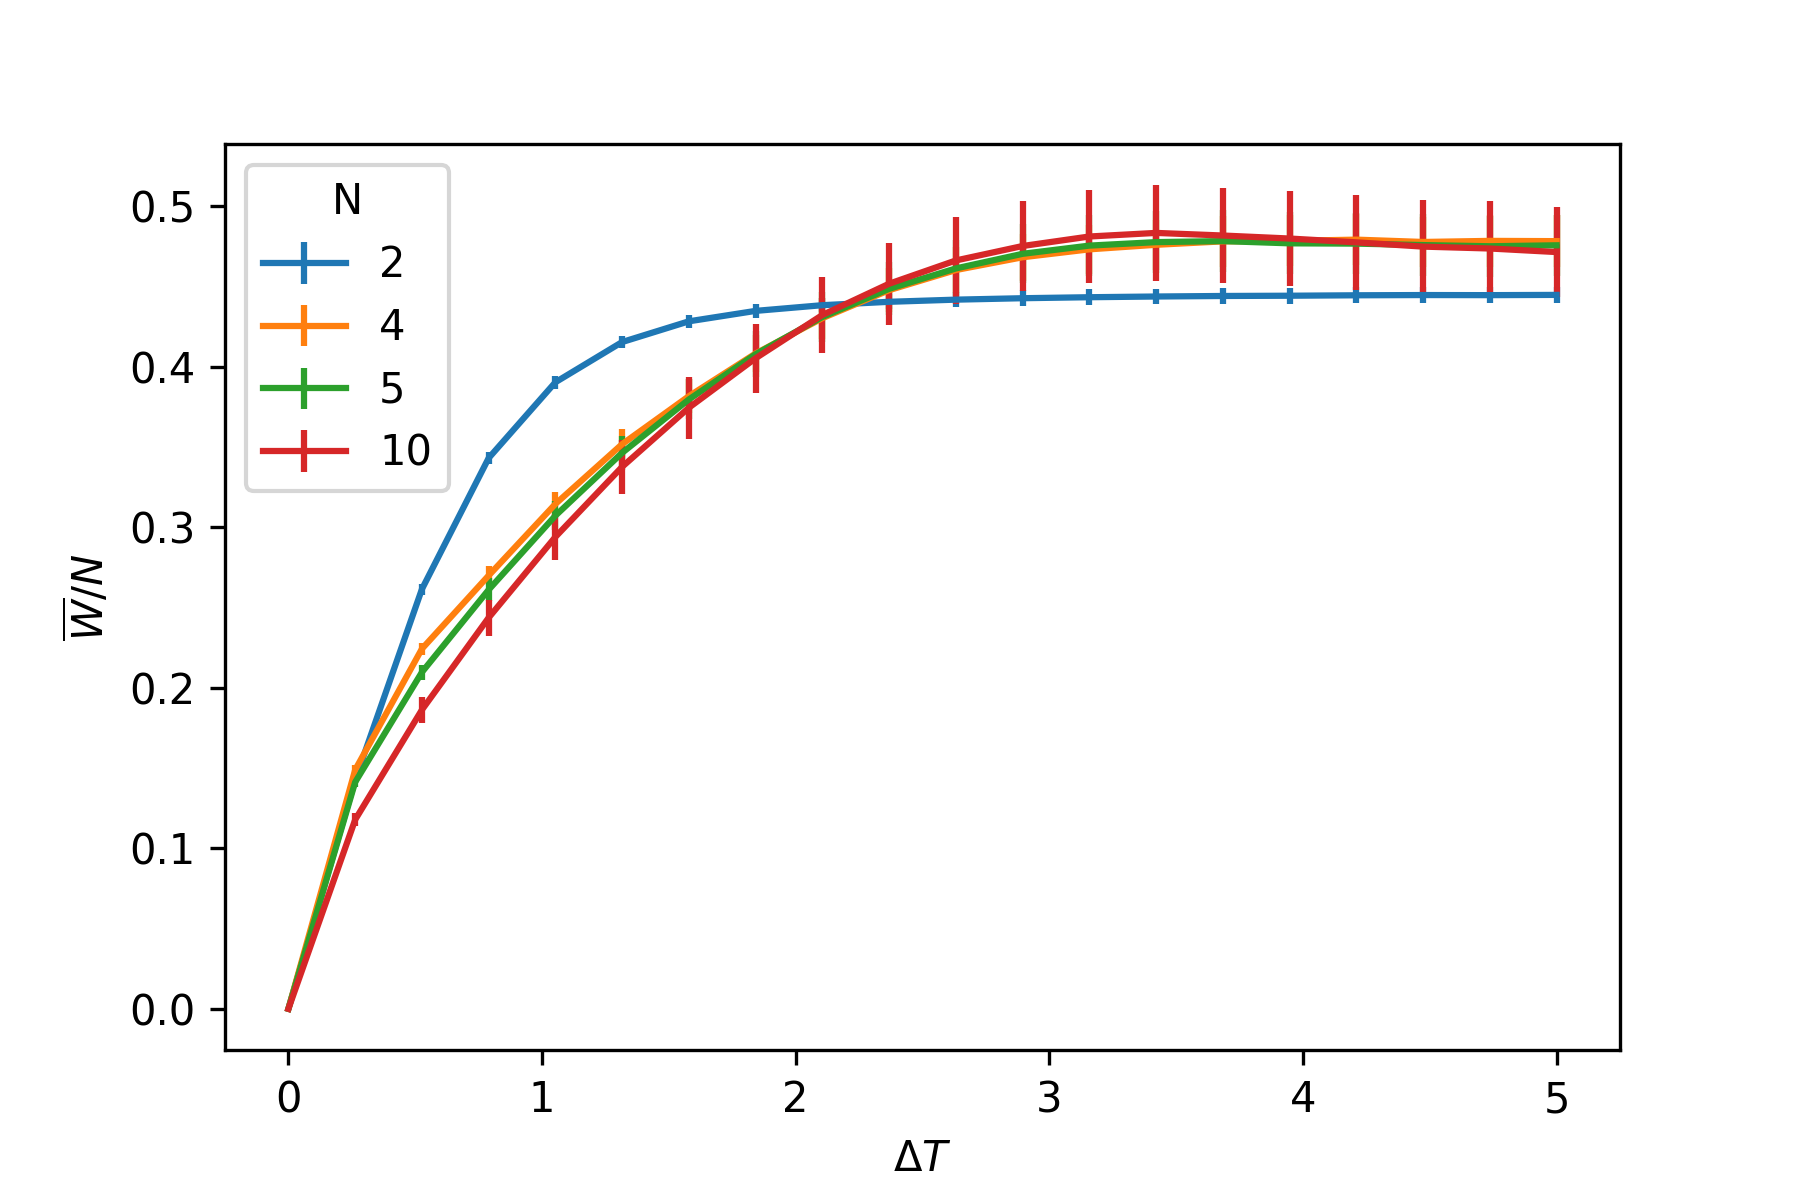
\includegraphics[width=\textwidth]{img/dt_0}
		\caption{$\rho_0 = \ket{0}\bra{0}$}
		\label{dt_0}
	\end{subfigure}
	\begin{subfigure}{0.4\textwidth}
	\centering
	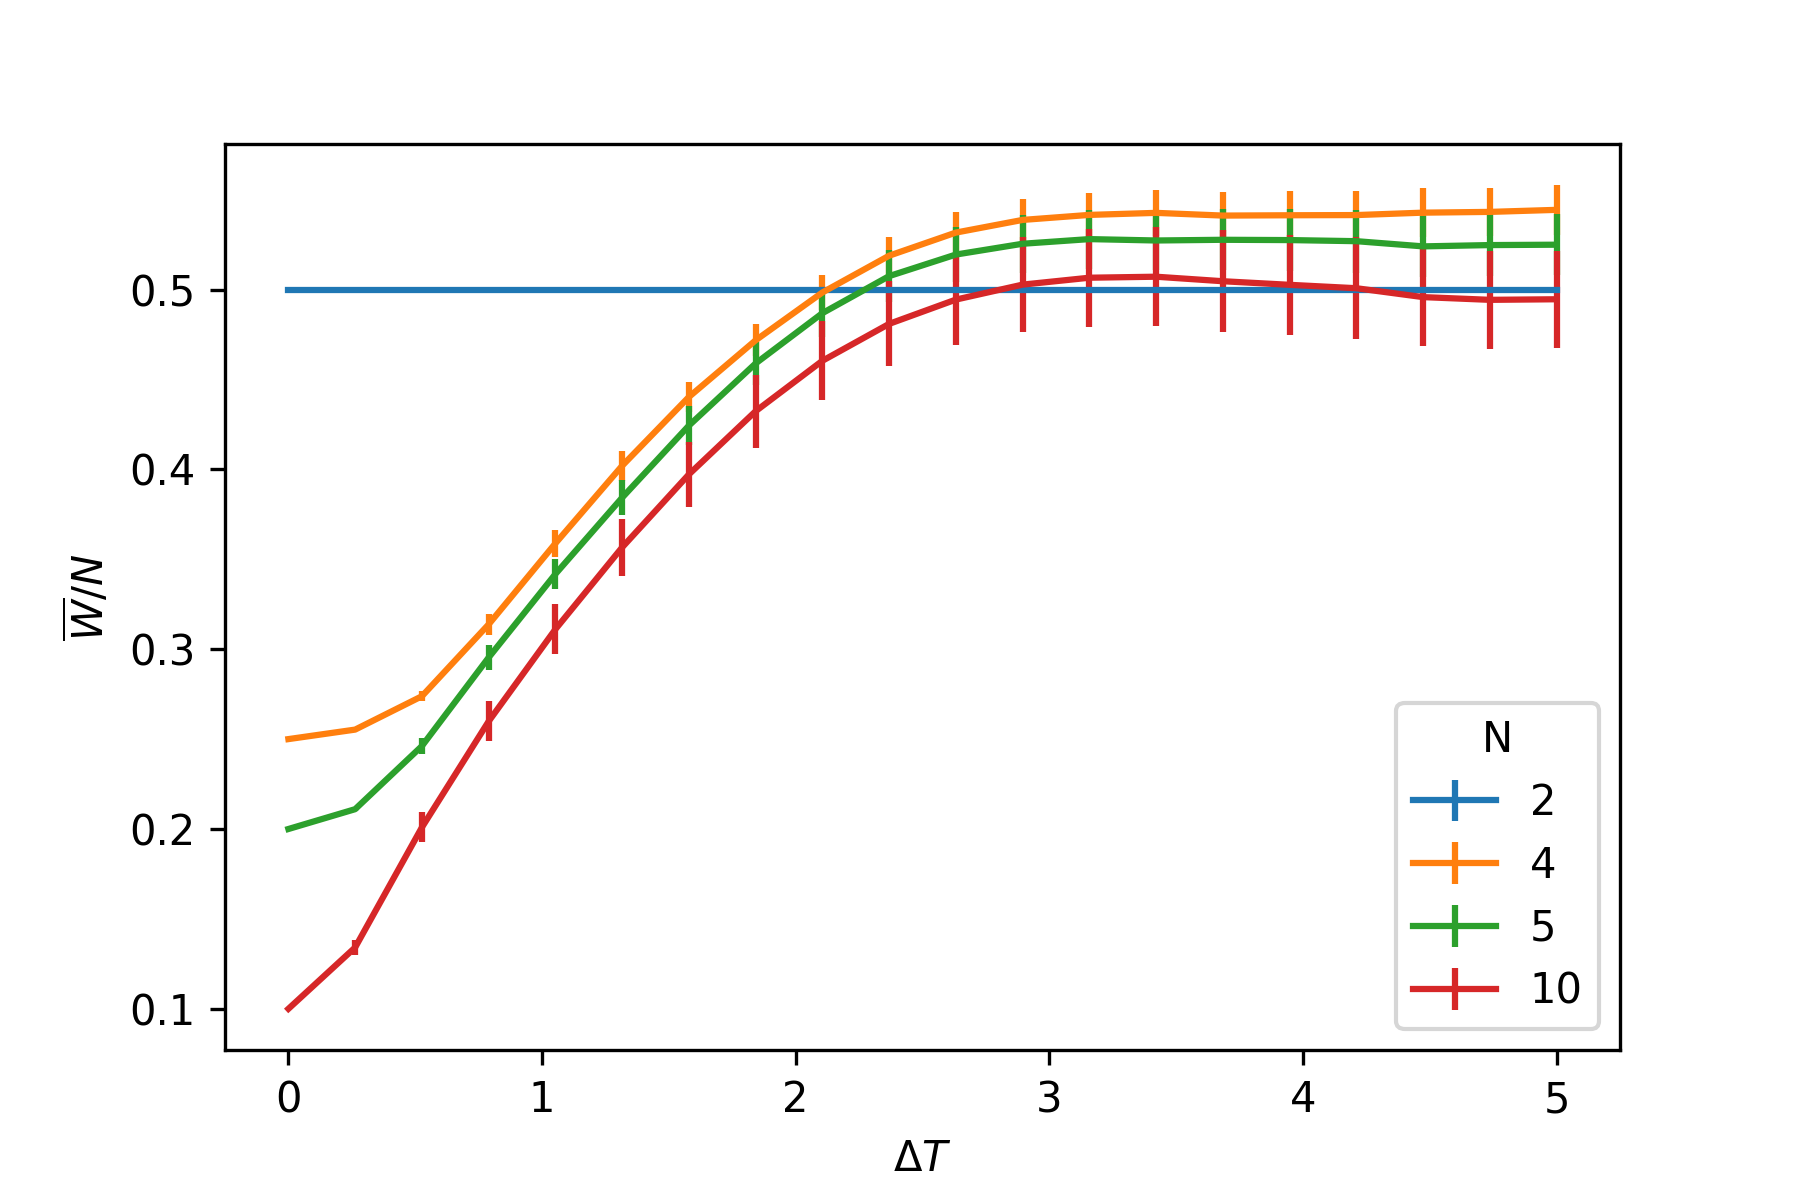
\includegraphics[width=\textwidth]{img/dt_eigen}
	\caption{$\rho_0 = \ket{+}\bra{+}$}
	\label{dt_eigen}
	\end{subfigure}
	\caption{(a) We plot the average work $\overline{W}$ over $n = 500$ runs of random excitations divided by amount of qubit changes $N - 1$, with $\rho_0 = \ket{0}\bra{0}$, for multiple $N$. The error bars correspond to the standard deviation $\sigma_{W} = \sqrt{\frac{1}{n-1} \Sigma_i^n (\overline{W} - W_i)^2}$.
	(b) We plot $\overline{W}/(N-1)$ for multiple $N$ where the system state is initialised in an eigenstate of the drive Hamiltonian $H_{DS}$.}
	\label{dt_dep}
\end{figure}
\section{$N=2$: Learning Single Jump Optimal Control Sequences} \label{n_2_ml}
% !TeX spellcheck = en_GB
For the simplest case of $N = 2$, we generate data sets of size $N_{\mathrm{data}} = 20000$ for $\rho_0 = \ket{0} \bra{0}, \ket{+} \bra{+}$ and random pure states.
The drive qubits are sampled randomly from the Haar measure \cite{Mezzadri}.
We train each data set on a fully-connected feedforward ANN with a single hidden layer with 10 neurons.
The efficiency of the models is presented in table \ref{n2efftable}.
For $N = 2$, starting in an eigenstate of the drive Hamiltonian $H_{DS}$ gives the highest model efficiency, as the optimal Transducer policy is trivial to learn and implement (see appendix \ref{n2_opt_pol}).

For random initial states the efficiency is close to zero.
This is to be expected, as without knowledge of the system state $\rho_0$ the optimal Transducer policy cannot be determined.\footnote{The deviation from zero is a relic of the way the test data is shuffled. For $N_{\mathrm{data}} \to \infty$ it would disappear.}
We therefore train the same network with the random initial state as additional inputs using the same embedding as the Drive sequence.
This increases the test data efficiency, but is still far below the efficiency for $\rho_0 = \ket{+} \bra{+}$.


\begin{table}[h]
	\centering
	\begin{tabular}{ c | c }
		$\rho_0$ & $\eta_{test} \ [\%]$ \\
		\hline
		$\ket{0} \bra{0}$ & 72.7 \\
		$\ket{+} \bra{+}$ & 100.0 \\
		Random & 0.5 \\
		Random, $\rho_0$ as input & 43.0 \\
	\end{tabular}
	\caption{Efficiencies $\eta$ on the test data for models with a single hidden layer with 10 neurons trained on drive protocols with $N = 2$ and differing initial states $\rho_0$.}
	\label{n2efftable}
\end{table}


%\begin{figure}
%	\centering
%	\begin{subfigure}{0.4\textwidth}
%		\centering
%		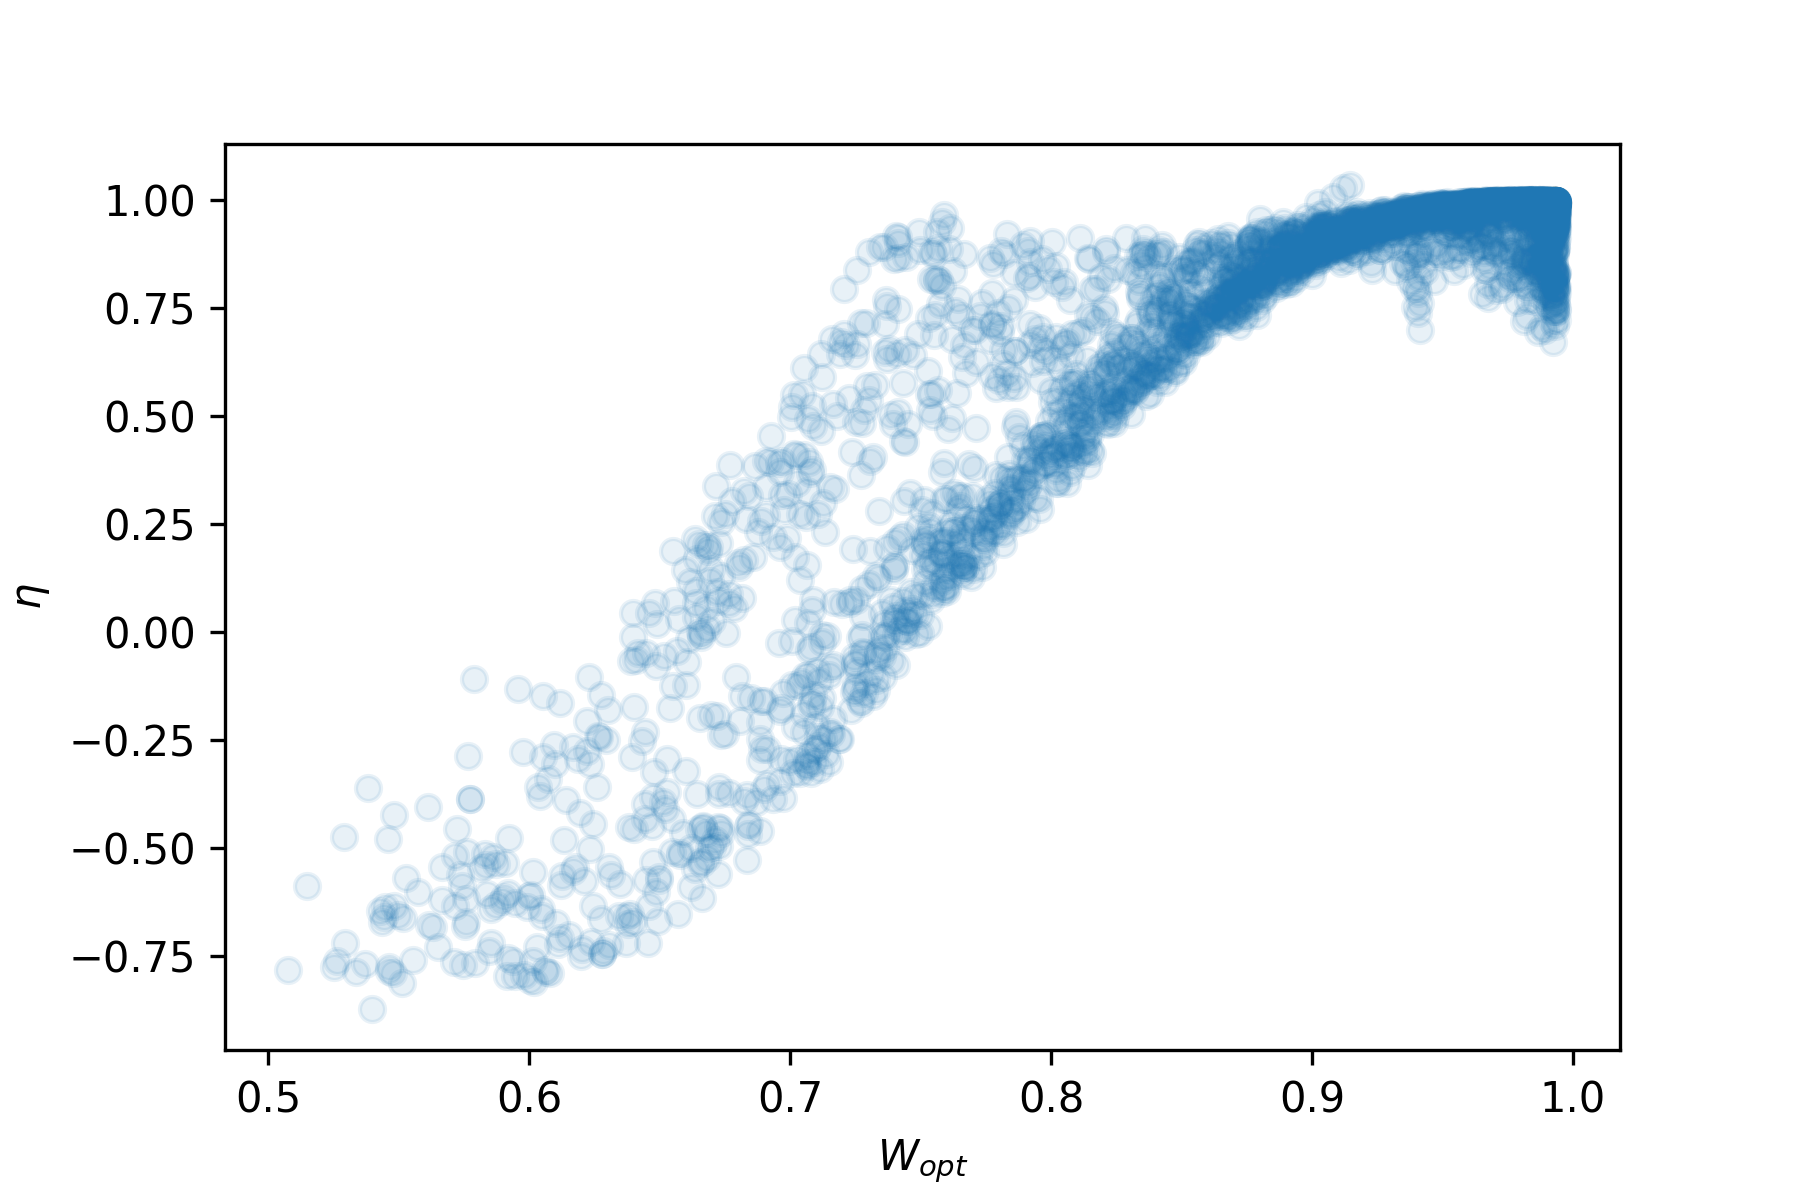
\includegraphics[width=\textwidth]{img/work_dist_n2_0}
%		\caption{$\rho_0 = \ket{0}\bra{0}$}
%		\label{}
%	\end{subfigure}
%	\begin{subfigure}{0.4\textwidth}
%		\centering
%		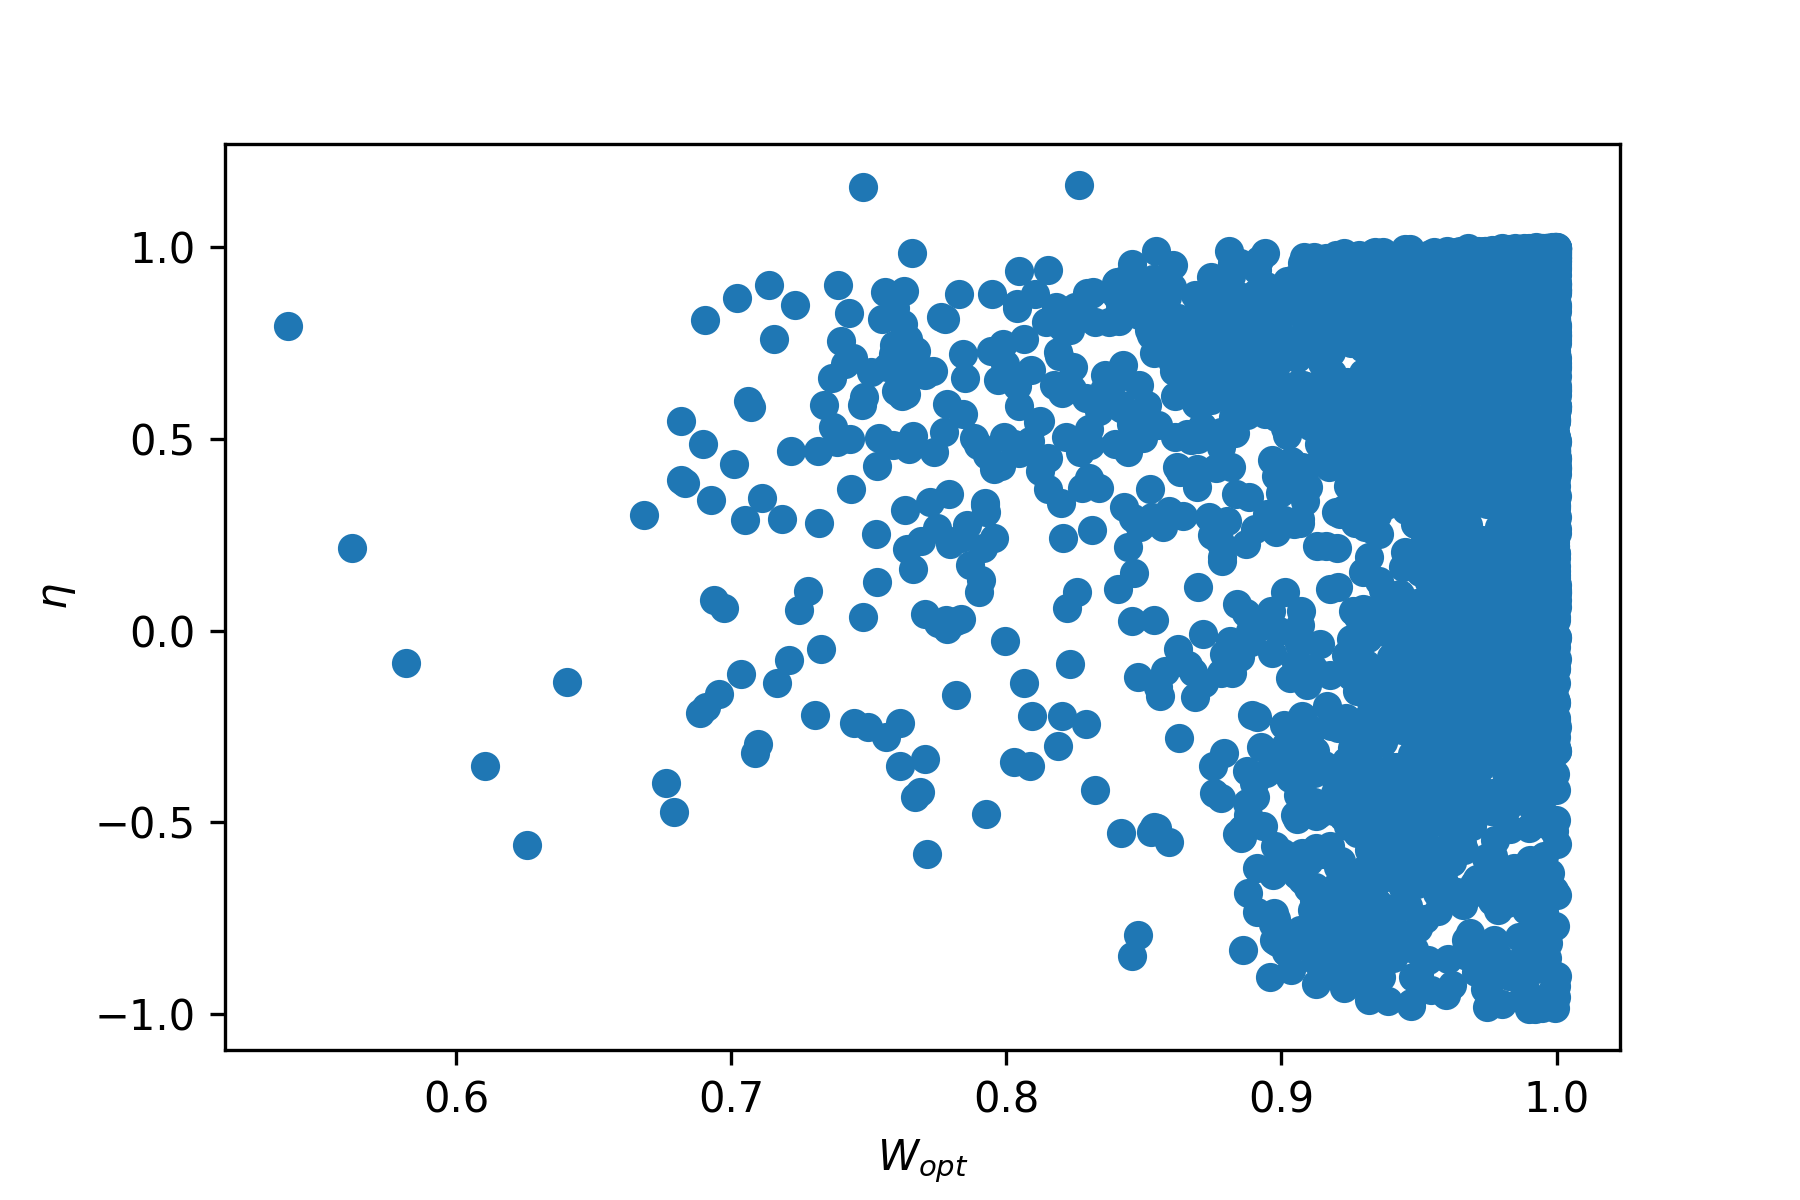
\includegraphics[width=\textwidth]{img/work_dist_n2_haar}
%		\caption{Random $\rho_0$}
%		\label{}
%	\end{subfigure}
%	\caption{}
%	\label{}
%\end{figure}
%
%
%\begin{figure}
%	\centering
%	\begin{subfigure}{0.4\textwidth}
%		\centering
%		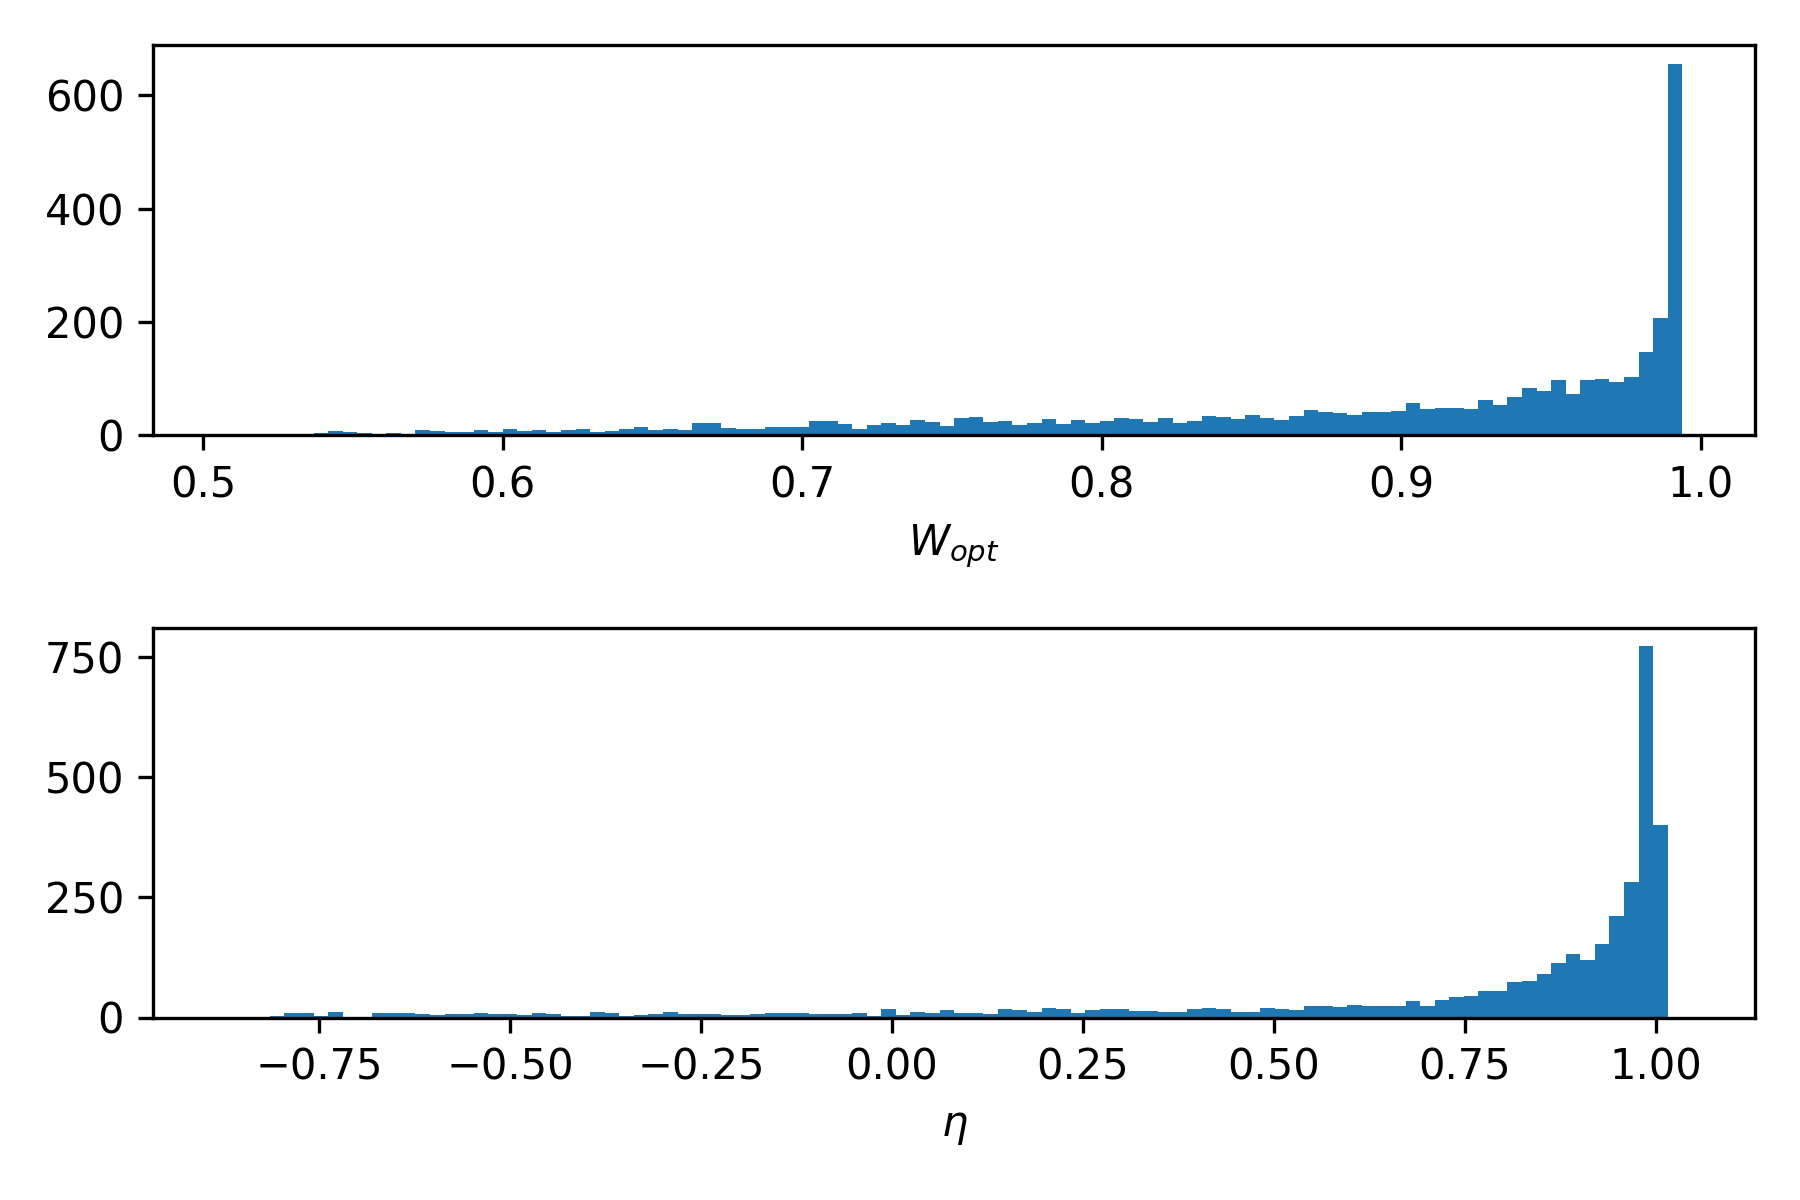
\includegraphics[width=\textwidth]{img/hist_n2_0}
%		\caption{$\rho_0 = \ket{0}\bra{0}$}
%		\label{}
%	\end{subfigure}
%	\begin{subfigure}{0.4\textwidth}
%		\centering
%		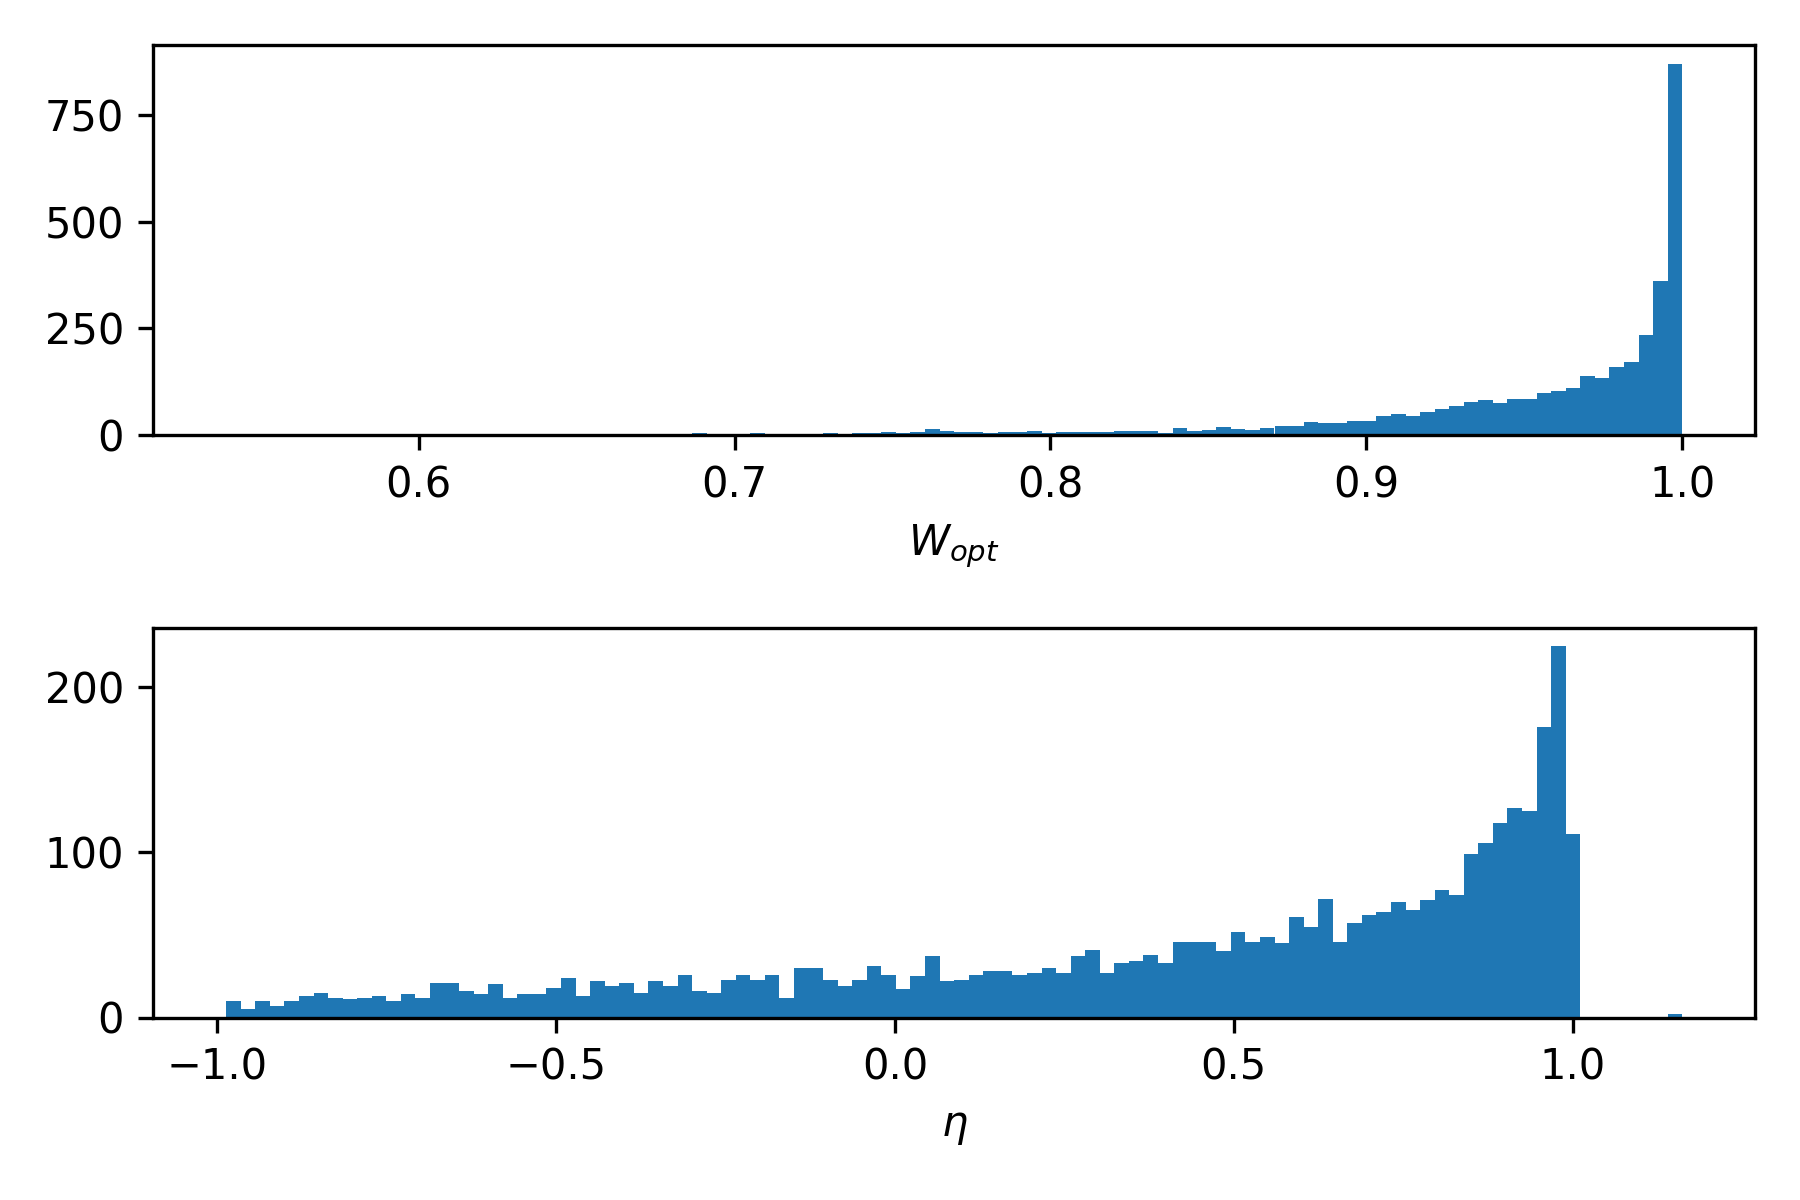
\includegraphics[width=\textwidth]{img/hist_n2_haar}
%		\caption{Random $\rho_0$}
%		\label{}
%	\end{subfigure}
%	\caption{}
%	\label{}
%\end{figure}

\chapter{Summary and Outlook}


\appendix
\chapter{Derivations}
\section{Single jump work output}
\begin{align*}
	H_S(\theta_D^t, \phi_D^t, \theta_T^t, \phi_T^t) & = \frac{1}{2} \left[\sin(\theta_D^t) e^{i\phi_D^t} + \sin(\theta_T^t) e^{i\phi_T^t}\right] \sigma_{+} + h.c. \\
	& = \alpha \sigma_{+} + h.c. \\
\end{align*}
\begin{align*}
	dH & = H_S(\theta_D^t, \phi_D^t, \theta_T^{t+1}, \phi_T^{t+1}) - H_S(\theta_D^t, \phi_D^t, \theta_T^t, \phi_T^t) \\
	& = \frac{1}{2}(\sin(\theta_T^{t+1})e^{i\phi_T^{t+1}} - \sin(\theta_T^t)e^{i\phi_T^t}) \sigma_{+} + h.c. =: (\tau' - \tau) \sigma_{+} + h.c. \\
\end{align*}
\begin{align*}
	U & = e^{-iH_S \Delta \mathrm{T}} = 
	\exp \begin{pmatrix}
	0 & -i\alpha^* \Delta \mathrm{T} \\
	-i \alpha \Delta \mathrm{T} & 0 \\
	\end{pmatrix}\\
	& = 
	\frac{1}{2} \begin{pmatrix}
	\frac{\alpha^*}{\abs{\alpha}} & -\frac{\alpha^*}{\abs{\alpha}} \\
	1 & 1 \\
	\end{pmatrix}
	\begin{pmatrix}
	e^{-i\abs{\alpha} \Delta \mathrm{T}} & 0 \\
	0 & e^{i\abs{\alpha} \Delta \mathrm{T}} \\
	\end{pmatrix}
	\begin{pmatrix}
	\frac{\abs{\alpha}}{\alpha^*} & 1 \\
	-\frac{\abs{\alpha}}{\alpha^*} & 1 \\
	\end{pmatrix} \\
	& = \begin{pmatrix}
	\cos(\abs{\alpha}\Delta \mathrm{T}) & -i\frac{\alpha^*}{\abs{\alpha}} \sin(\abs{\alpha}\Delta \mathrm{T}) \\
	-i\frac{\abs{\alpha}}{\alpha^*} \sin(\abs{\alpha}\Delta \mathrm{T}) & \cos(\abs{\alpha} \Delta \mathrm{T}) \\
	\end{pmatrix} \\
\end{align*}
	With $\ket{\psi_0} = a \ket{0} + b \ket{1}$,  $\abs{a}^2 + \abs{b}^2 = 1$, we  have
\begin{align*}
	\rho_0 & = \begin{pmatrix}
	\abs{a}^2 & a b ^* \\
	a^* b & \abs{b}^2 \\
	\end{pmatrix}, \ \rho = U \rho_0 U^\dagger = 
	\begin{pmatrix}
	\rho_{00} & \rho_{01} \\
	\rho_{10} & \rho_{11} \\
	\end{pmatrix}  \\
	\rho_{00} & = \abs{a}^2 \ \cos^2(\abs{\alpha} \Delta \mathrm{T}) + \abs{b}^2 \ \sin^2(\abs{\alpha} \Delta \mathrm{T}) - \frac{1}{\abs{\alpha}} \sin(2 \abs{\alpha} \Delta \mathrm{T}) \Im{a b^* \alpha} \\
	\rho_{01} & = \frac{\alpha^*}{2 \abs{\alpha}} i \ \sin(2 \abs{\alpha} \Delta \mathrm{T}) (\abs{a}^2 - \abs{b}^2) + \frac{\alpha^*}{\alpha} a^* b \sin^2(\abs{\alpha} \Delta \mathrm{T}) + a b^* \ \cos^2(\abs{\alpha} \Delta \mathrm{T}) \\
	\rho_{10} & = 	\frac{\abs{\alpha}}{2 \alpha^*} i \ \sin(2 \abs{\alpha} \Delta \mathrm{T}) (\abs{b}^2 - \abs{a}^2) + \frac{\alpha}{\alpha^*} a b^* \ \sin^2(\abs{\alpha} \Delta \mathrm{T}) + a^* b \ \cos^2(\abs{\alpha} \Delta \mathrm{T}) \\
	\rho_{11} & = \abs{a}^2 \ \sin^2(\abs{\alpha} \Delta \mathrm{T}) + \abs{b}^2 \ \cos^2(\abs{\alpha} \Delta \mathrm{T}) + \frac{1}{\abs{\alpha}} \sin(2 \abs{\alpha} \Delta \mathrm{T}) \Im{a b^* \alpha}
\end{align*}
\begin{align*}
	\mathrm{dW} = & - \mathrm{Tr} \ \rho \ \mathrm{dH} = \frac{\abs{a}^2 - \abs{b}^2}{\abs{\alpha}} \sin(2 \abs{\alpha} \Delta \mathrm{T}) \Im{(\tau' - \tau) \alpha^*} \\
	& - 2 \ [\cos^2(\abs{\alpha} \Delta \mathrm{T}) \Re{(\tau' - \tau) a b^*} 
	+ \sin^2(\abs{\alpha} \Delta \mathrm{T}) \Re{(\tau' - \tau)a^* b \frac{\alpha^*}{\alpha}} ]
\end{align*}

\section{Optimal ? policy for $N=2$} \label{n2_opt_pol}
For $\rho_0 = \ket{+} \bra{+}$, or $a = e^{-i \phi_D}/\sqrt{2}, b = 1/\sqrt{2}$ following the notation used in appendix \ref{deriv_jump}, finding the optimal solution of $\mathrm{dW}$ for $N = 2$ requires finding the transducer setting that ensures
\begin{align}\label{commutator}
	[H_{DS}, H_S] = [\delta \sigma_{+} + \delta^* \sigma_{-}, \alpha \sigma_{+} + \alpha^* \sigma_{-}] = 0
\end{align}
with $\delta = \frac{1}{2} \sin{\theta_D} e^{i \phi_D}$.
\ref{commutator} is equivalent to
\begin{align*}
	\Im{\alpha \delta^*} = 0 \implies \arg{\alpha} = \phi_D \implies a b^* = a^* b \frac{\alpha^*}{\alpha},
\end{align*}
which leads to the independence of dW with regard to $\Delta \mathrm{T}$. 
\chapter{Training protocols}
% !TeX spellcheck = en_GB
In all models we split the data into training, validation and test data with $p_{test} = 18 \%$ and $p_{valid} = 8.2 \%$. 
The models are implemented using the PyTorch library \cite{NEURIPS2019_9015}. 
Training is performed over $n$ epochs, in each of which the complete training set is used once in batches of \textit{batch size}.
In each batch, the gradient of the loss function with regard to the model parameters is calculated.
The gradient average over the data points in a batch are used to update the trainable parameters.
We use early stopping to stop training when the value of the cost function on the validation set does not improve for \textit{patience} epochs.
We apply dropout \cite{hinton2012improving} after all layers except for input and output.

\section{Hyperparameters Section \ref{n_2_ml}}
For $N=2$, we use the Adam optimiser with $\beta_1 = 0.9$, $\beta_2 = 0.98$ and $\epsilon = 10^{-9}$. The learning rate (LR) is determined by an exponential decay schedule
\begin{equation} \label{eds}
\mathrm{LR} \ (i) = \mathrm{initial \ LR} * \mathrm{decay \ rate}^i,
\end{equation}
where $i$ denotes the optimiser step.


\begin{table}[h]
	\centering
	\begin{tabular}{c | c | c }
		Patience & Initial LR & Decay Rate \\
		\hline
		100 & $10^{-2}$ & 0.995 \\
	\end{tabular}
	\caption{Hyperparameters used in training for the models in section \ref{n_2_ml}.}
	\label{hyperparams_n_2}
\end{table}

\section{Hyperparameters Sections \ref{n_5_ml} and \ref{n_5_dt1}}
The learning rate (LR) is determined by the `Reduce LR on Plateau' schedule.
The learning rate is multiplied by the hyperparameter \textit{factor} when the cost function does not improve for \textit{patience} / \textit{pat drop} epochs.
The hyperparameters are found using Bayesian optimisation implemented by \cite{wandb} and can be found in Table \ref{hyperparams_n_5}.
The FCANN in Section \ref{n_5_ml} has three hidden layers with 2000 neurons each.

\begin{table}[h]
	\centering
	\begin{tabular}{l | l}
		Hyperparameter & Value \\
		\hline
		Optimiser & SGD \\
		Batch size & 44 \\
		Dropout & 0.3179732914255167 \\
		Input layer 1 size & 793 \\
		Input layer 2 size & 488 \\
		Output layer size & 228 \\
		LSTM hidden size & 324 \\
		Large hidden size in Section \ref{n_5_dt1} & 552 \\
		Initial learning rate & 0.02847560288866327 \\
		LSTM layers & 3 \\
		Pat drop & 3.698498258242224 \\
		Patience & 55 \\
		Factor & 0.24509238889070978
	\end{tabular}
	\caption{Hyperparameters used for the models in Sections \ref{n5} and \ref{work_cost}.}
	\label{hyperparams_n_5}
\end{table}


\bibliographystyle{plain}
\bibliography{biblio}



% Erklärung
\clearpage
\thispagestyle{empty}
\minisec{Erklärung}\vspace*{1.5em}

Hiermit erkläre ich, dass ich diese Arbeit im Rahmen der Betreuung am Institut
für Theoretische Physik ohne unzulässige Hilfe Dritter verfasst und alle Quellen als solche gekennzeichnet habe.

\vspace*{45em}

Felix Soest \par
Dresden, Monat 2021

\end{document}
